% !TEX root = main.tex
\label{ch:campaigns}
Computational campaigns enact an execution plan to achieve a computational objective under given requirements and constraints.
The computational objective is a set of values selected by the user for a set of metrics.
Some of these metrics are time to completion and throughput.
Requirements, generally, describe the minimum amount and type of resources needed to execute each workflow of the campaign, while the constraints are the conditions that bound the execution, such as resource availability, resource capacity or costs.

The objective of a campaign can be translated to a computational objective function that would either minimize or maximize a metric.
Among the many metrics that could be considered, the most common one is the total time taken to execute all workflows of a campaign, also known as makespan.
An execution plan of a campaign is a mapping between workflows and resources to execute upon.
Calculating the makespan of a campaign means finding an execution plan that satisfies the computational objective function.

A computational campaign can utilize several resources concurrently.
These resources can either be homogeneous or heterogeneous as they offer different type of computational resources.
One aspect of this heterogeneity is the performance each resource has in terms of number of operations per second.
High Performance Computing (HPC) resources, a campaign can utilize, offer the concurrent execution of workflows on different sets of the same type or different type of computational resources, thus homogeneous or heterogeneous respectively.
Different types of computational resources can be offered by the same HPC resource or different HPC resources.

During the execution of a campaign, uncertainty can arise for several reasons, including resource dynamism and workflow runtime uncertainty.
HPC resources are governed via policies that affect their performance, such as power regulating policies~\cite{inadomi2015analyzing} and filesystem and network  multitenacy~\cite{brown2018interference}.
As a consequence, their performance changes over time and is dynamic, which in turn creates uncertainty on the makespan of a campaign.
Further, accurately estimating the runtime of each workflow in a campaign is challenging, as each workflow can have different inputs or datasets to analyze.
Instead, users offer an estimation in the form of a range of possible values.
Both resource dynamism and workflow runtime uncertainty have the potential to increase the makespan of an execution plan.

There is a plethora of algorithms which derive an execution plan by calculating the makespan of a workflow, and not a campaign, offline~\cite{lu2019review}, i.e., before the execution of a workflow.
Selecting and extending an algorithm that is suitable to plan the execution of a campaign on HPC resources is not trivial.
To the best of our knowledge, there is not a methodology that allows to compare planning algorithms and select the most suitable for planning the execution of a campaign on a set of resources.
We select three algorithms that each represents a larger family and compare their performance in respect to the makespan of the plans they produce as well as how sensitive they are on resource dynamism and workflow runtime uncertainty.
Based on the comparison, we make a case of which algorithm to select given a computational campaign, its requirements and constraints.

The chapter offers the following contributions:
\begin{inparaenum}[i)]
    \item an experiment-based methodology to compare planning algorithms performance that is independent of the considered use case and computing framework;
    \item a conceptual framework for selecting planning algorithms based on the algorithmic, campaign and resources characteristics
\end{inparaenum}

The chapter is organized as follows: \S~\ref{sec:makespan_calc} discusses the calculation of the makespan of a campaign given the set of assumptions of this work.
Section \S~\ref{sec:algo} discusses three selected makespan calculation algorithms and \S~\ref{sec:algo_perf_comp} compares their performance.
Finally, section \S~\ref{sec:cf_algo_sel} presents our conclusions and a conceptual framework that will allow users to best select a planning algorithm.

% -------------------------------------------------------------------
\section{Calculating the Makespan of a Campaign}
\label{sec:makespan_calc}
The way workflows of a given campaign are mapped to resources can affect the makespan calculation. 
Figure~\ref{fig:example_makespan} shows an example of a campaign with workflows of different size and execution times, and the makespans that two different mappings produce.
The makespan of the campaign on the left sub~-figure is $20$, while on the right it is $16$.
In addition, the size of the workflows, i.e., the number of resources they require, becomes relevant and resources may be underutilized, as shown in Figure~\ref{fig:example_makespan}.

\begin{figure*}[ht!]
    \centering
    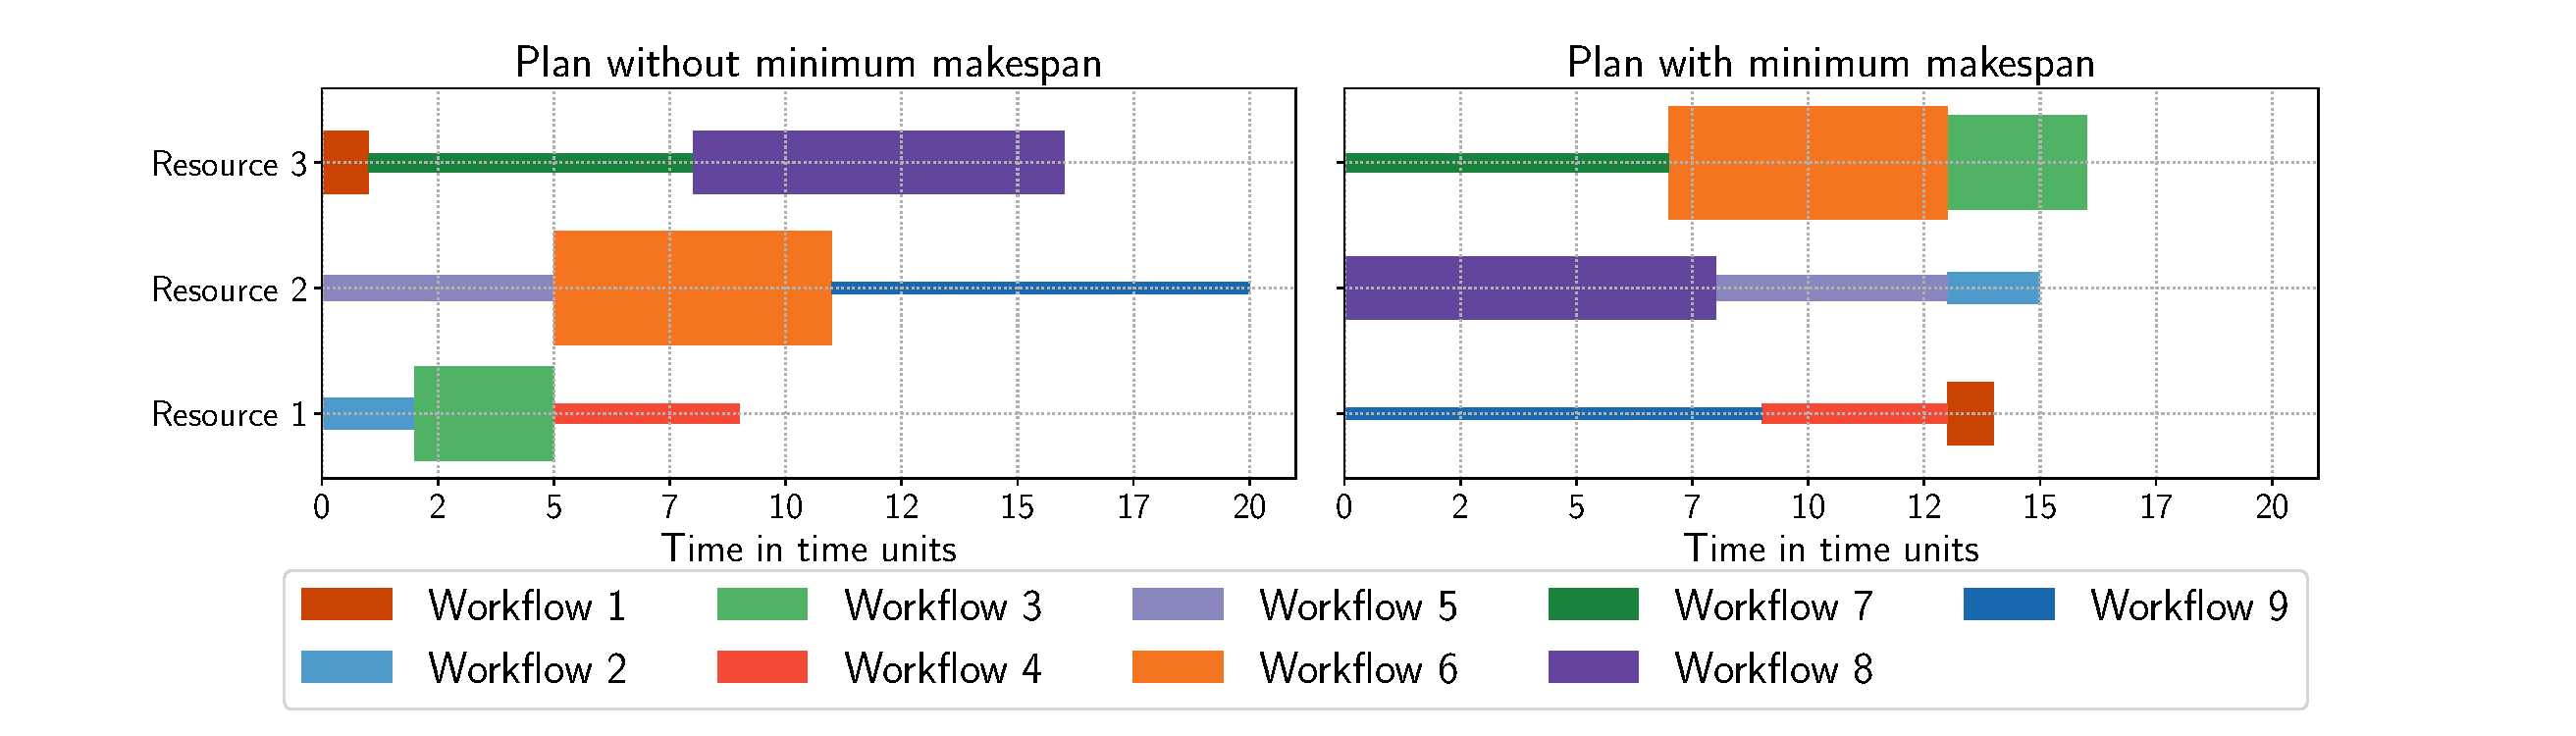
\includegraphics[width=.99\textwidth]{figures/campaign/plan_comp.pdf}
    \caption{Comparison of different campaign execution plans. Based on workflow mapping on resources makespan and resource utilization is different.}\label{fig:example_makespan}
\end{figure*}

We are making a set of assumptions which we do not relax during the analysis of a model that calculates the makespan of a campaign.
These are:
\begin{inparaenum}[(1)]
    \item a workflow is an atomic unit and cannot be decomposed;
    \item workflow resource request is sufficient to execute the workflow;
    \item a resource is an aggregate of computing capabilities;
    \item every workflow of a given campaign can be executed on the given resources;
    \item random resource selection is based on a uniform distribution;
    \item only one workflow can be executed on a resource at any point in time; and
    \item workflows can be homogeneous or heterogeneous in time---the amount of time they are executing--- and space---the amount of resources they require.
\end{inparaenum}

We denote a computational campaign as $C = [w_{i}: 1 \leq i \leq N_{C}]$, where $w_{i}$ is a workflow and $N_{C}$ is the total number of workflows, $R = [ r_{j}: 1 \leq j \leq N_{R}]$ is a set of available resources, where $r_{j}$ is a resource and $N_{R}$ is the total number of available resources, and $ M(C,R) = [(w_i, r_j): 1 \leq i \leq N_{C}, r_j \in R] $ is a mapping function of workflows onto resources.
In addition, we denote the execution time of a workflow as $Tx_{w_{i}}$, the makespan of campaign $C$ as $TTX_{C}$, and the makespan of campaign $C$ for a given mapping function $ M $ as $TTX_{C}(M)$.
Assumption~\#3 allows to abstract the resource implementation details, as workflows can be executed on different resources such as HPCs, Clouds, pilots and more. 

With a single resource, i.e., $N_{R} = 1$, the workflows of a campaign will be executed sequentially, regardless the execution order or whether the workflows are homogeneous or heterogeneous.
As a result the makespan of the campaign is:
\begin{equation}
   TTX_{C} = \sum_{i=1}^{N_{C}}Tx_{w_{i}} 
\end{equation}

With multiple resources, i.e., $1 < N_{R} < N_{C}$, the workflows of a campaign can be executed concurrently.
With homogeneous resources, this is semantically equivalent to executing on a single resource large enough to allow concurrent workflow execution, where each workflow executes on a resource partition. 
Because of assumptions~\#4 and~\#7, executing homogeneous or heterogeneous in space workflows has the same makespan.
A random mapping of workflows onto resource will have a makespan:
\begin{equation}
   TTX_{C}(Random) \geq \frac{1}{N_{R}}\sum_{i=1}^{N_{C}} Tx_{w_{i}} 
\end{equation}
Given multiple homogeneous resources, when executing workflows that are heterogeneous in time and that can be homogeneous or heterogeneous in space, the makespan of the campaign for a given mapping function $ M $ is:
\begin{equation}
TTX_{C}(M) = \max_{r_{j}\in R}\Big\{\sum_{w_{i}\in M(C,r_{j})}Tx_{w_{i}}\Big\}
\label{eq:makespan}
\end{equation}
Relaxing the assumption that resources are heterogeneous, in the performance they offer, affects the result of the mapping function $ M $.
As a result, Eq.~\ref{eq:makespan} holds in calculating the makespan of the campaign.

Computational campaigns execute to achieve an objective.
We consider as objective the total time of completion of the campaign.
As a result, the objective function of a plan is translating in minimizing the value of eq~\ref{eq:makespan}.
As objective function is:
\begin{equation}
    \min\Big\{\max_{r_{j}\in R}\Big\{\sum_{w_{i}\in M(C,r_{j})}Tx_{w_{i}}\Big\}\Big\}
\end{equation}
In the next section, we discuss a set of algorithms that try to satisfy this objective function.

% -------------------------------------------------------------------
\section{Planning Algorithms}
\label{sec:algo}

As mentioned before, there is a plethora of methods and algorithms to calculate the makespan of a workflow~\cite{lu2019review}.
%, including queuing networks~\cite{yao2019throughput,bao2019performance}, domain specific languages~\cite{carothers2017durango,maheshwari2016workflow}, and machine learning~\cite{witt2019predictive,pumma2017runtime}.
From this plethora of selections, we selected to investigate and extend three algorithms, each one representative of a larger family of algorithms.
The algorithms are Heterogeneous Earlier Finish Time algorithm (HEFT)~\cite{topcuoglu2002performance}, a genetic algorithm~\cite{page2005algorithm} and a simple heuristic algorithm.
As all these algorithms are producing an execution plan before the actual execution of the campaign, they require workflow runtime and resource performance as input.
Table~\ref{tab:sched_algo} shows a summary of the algorithms characteristics.

\begin{table}[t]
    \centering
    \scriptsize
    \begin{tabular}{@{}ccccc@{}}
        \toprule
        &\textbf{HEFT}     &\textbf{Genetic Algorithm} &\textbf{L2FF} & \textbf{Random} \\
        \midrule
        Decision Policy   &Deterministic &Convergence Criteria &Deterministic& Deterministic\\
        Initial State    &Blank &Semi-random &Blank & Blank\\
        \midrule
        \multicolumn{5}{l}{\textbf{Initial Information}}\\\midrule
        Workflow Operations &Yes & Yes & Yes & No\\
        Resource Performance &Yes &Yes &Yes & No\\
        \midrule
        Produced Knowledge& Resource availability& Resource availability&None&None\\
        \bottomrule
    \end{tabular}
    \caption{Basic characteristics of selected planning algorithms.\label{tab:sched_algo}}
\end{table}

% -------------------------------------------------------------------
\subsection{Heterogeneous Earlier Finish Time (HEFT) algorithm}
\label{algo:heft}
List scheduling algorithms represent a general family of heuristic based scheduling algorithms to schedule workflows described as direct acyclic graphs~\cite{dong2006scheduling,list_sched_wiki}. 
These algorithms assign priorities to tasks based on a heuristic and order them.
Then, they traverse the list of tasks and assign tasks to resources.
HEFT is an example of this type of algorithms~\cite{dong2006scheduling} and calculates the makespan of a workflow on heterogeneous resources, in terms of performance.

HEFT has been implemented as part of the planning capabilities in Pegasus~\cite{deelman2015pegasus} and ASKALON~\cite{fahringer2005askalon} amongst other algorithms.
HEFT has been shown to provide better performance in terms of makespan minimization compared to other mapping algorithms,~\cite{topcuoglu2002performance,canon2008comparative}, e\.g\., genetic algorithms~\cite{fahringer2005askalon}. 
Furthermore, there has been some initial research to extend HEFT to resources that provide CPU and GPUs~\cite{shetti2013optimization} and on dynamic resources~\cite{dong2007pfas}. 

HEFT makes two important assumptions when used on workflows: 
\begin{inparaenum}[(1)] 
    \item any task in a workflow can be executed on all available resources; and 
    \item all resources are initially available.
\end{inparaenum}
Note that assumption~\#1 is equivalent to assumption~\#4 in \S~\ref{sec:makespan_calc}.
HEFT's complexity is proportional to the number of dependencies between tasks and the number of resources offered. 
As we are interested in executing computational campaigns, our HEFT extension provides an execution plan based on workflows as atomic units instead of tasks.
Algorithm~\ref{alg:heft} shows HEFT for placing independent workflows on resources.

\begin{algorithm}[t]
    \caption{Heterogeneous Earliest Finish Time (HEFT) algorithm}
    \label{alg:heft}
    \scriptsize
    \begin{algorithmic}[1]
        \Procedure{HEFT}{$W$,$R$}\Comment{$W$ and $R$ are a set of workflows and resources respectively}
        \State \texttt{Calculate the computation cost $w_{tx}^{ij}$ of each workflow for all resources}
        \State \texttt{Assign $rank_i = \overline{w_{i}} = \nicefrac{\sum_{j=1}^{|R|}w_{tx}^{ij}}{|R|}$}
        \State \texttt{Sort workflows in decreasing order of $rank_i$}
        \While{unscheduled workflows}
        \State \texttt{Select the first workflow $\tilde{w}$ from the sorted list}
        \For{$\forall r_{j}$ in $R$}
        \State\texttt{Compute earliest finish time for $\tilde{w}$ on $r_{j}$, $eft_{\tilde{w},r_j}$ }
        \EndFor
        \State \texttt{Assign  $\tilde{w}$ on $r_k$ with $\min{(eft_{\tilde{w},r_j})}$}
        \EndWhile
        \EndProcedure
    \end{algorithmic}
\end{algorithm}

HEFT has three main algorithmic characteristics:
\begin{inparaenum}[1)]
    \item creates a priority list of workflows,
    \item produces an expectation of when resources are available and
    \item uses a deterministic heuristic.
\end{inparaenum}
HEFT initially calculates the average execution time of a workflow on all resources and creates a priority list with the longest workflow first.
In addition, HEFT initializes a vector where each element is when a resource is available.
Then, HEFT calculates when a workflow will finish at each resource and places the workflow on the resource that will finish it earlier.
HEFT ends when all workflows are placed on a resource.

   
% -------------------------------------------------------------------
\subsection{Genetic Algorithm}
\label{algo:gen}
Genetic algorithms represent another family of algorithms that are used to calculate the makespan of workflows~\cite{dong2006scheduling}.
Genetic algorithms start from an initial set of possible solutions, iterate and improve them at every iteration.
In general, genetic algorithms follow the following procedure:
\begin{inparaenum}[(i)]
    \item create an initial population, where the population is a set of possible plans;
    \item evaluate the population members based on a fitness function, which calculates the makespan of the workflow;
    \item reproduce by selecting population members, either randomly or based on their fitness value, and generate a new set of possible plans; and
    \item mutate, where randomly selected tasks from a random population member are reassigned to resources.%; and
%    \item re-evaluate the members in the population to check convergence.
\end{inparaenum}

The selected genetic algorithm~\cite{page2005algorithm} is developed to support the placement of independent tasks on heterogeneous resources.
It assumes that all tasks can be executed on all available resources, are independent and indivisible.
These assumptions are in accordance with the assumptions made for workflows in a campaign.
We extend this algorithm can be extended to support scientific campaigns.
The pseudocode of the selected genetic algorithm is shown in Algorithm~\ref{alg:gen_algo}.

\begin{algorithm}[t]
    \caption{Genetic Algorithm}
    \label{alg:gen_algo}
    \scriptsize
    \begin{algorithmic}[1]
        \Procedure{GA}{$W$, $R$}\Comment{$W$ and $R$ are a set of workflows and resources respectively}
        \State \texttt{Initaliaze population}
        \While{Conergence Criteria not met and \#Gen $<$ Total\_Generations}
        \State{Selection}
        \State{Reproduce}
        \State{Randomly mutate}
        \EndWhile
        \EndProcedure
    \end{algorithmic}
\end{algorithm}

The members of the initial population are constructed either randomly or semi-randomly.
Specifically, a percentage of the workflows are assigned randomly to resources, where the assignment is drawn by uniform distribution and the rest of the workflows are assigned based on an earlier finish time (EFT) heuristic, similar to the one used by HEFT.
The population size is relatively small to 20 members, i.e., potential plans, called micro-GA.
Micro-GA has been shown to reduce the computational load of the genetic algorithm and not significantly impact the final result~\cite{zomaya2001observations}.

The genetic algorithm uses a fitness function to calculate the goodness, or fitness, of a population member or plan, returning a value between 0 and 1.
The fitness function calculates the distance of a plan from the ideal makespan.
This distance is defined as:
\begin{equation}
E = \sqrt{(\sum_{j=1}^{N_{C}}Tx_{w_{j},r_{j}} - IM)^2}
\label{eq:fitness}
\end{equation}
where $N_{C}$ is the number of workflows and $IM$ is the ideal makespan.
The ideal makespan is equal to
\begin{equation}
IM = \frac{\sum_{i=1}^{N_{C}}Tx_{w_{i}}}{\sum_{j=1}^{N_{R}}r_{j}}
\label{eq:ideal_fitness}
\end{equation}
The fitness of a plan is the equal to $F = 1 /E$ when $E > 0$, otherwise to 1.

The algorithm selects members to reproduce based on their fitness values.
Each member fitness value defines the probability of that member to be selected.
When the selection is complete the algorithm uses cyclic rotation~\cite{oliver1987study} to generate new population members and replaces those with the lowest fitness.
After a population member is selected randomly and two random workflows swap, completing the mutation step.
The algorithm stops evolving either when a member has fitness equal to 1 or after a specified number of iterations.

The genetic algorithm has the following algorithmic characteristics:
\begin{inparaenum}[1)]
    \item creates partial plans randomly,
    \item produces an expectation of when resources are available,
    \item evolves plans randomly and
    \item terminates based on a convergence criteria
\end{inparaenum}


% -------------------------------------------------------------------
\subsection{Longest to Fastest First Available Resource Algorithm}
\label{algo:l2ff}
The last algorithm is a simple heuristics algorithm.
It places workflows based on the rule: largest workflow to fastest first available resource (L2FF)~\cite{balasubramanian2019programming}.
This algorithm sorts the workflows based on the number of operations, or workflow runtime estimation, and resources based on their performance.
Then it places each workflow on the first fastest available resource.
A resource is considered available when it has less or equal number of workflows than any other resource.
When workflows and resources are sorted, the placement is equivalent to a modulo operation between the position of the workflow in the sorted list with the number of resources.
Algorithm~\ref{alg:l2ff} show the pseudocode for this algorithm.

\begin{algorithm}[ht]
    \caption{Longest to Fastest First (L2FF)}
    \label{alg:l2ff}
    \begin{algorithmic}[1]
        \Procedure{l2ff}{$W$, $R$}\Comment{$W$ and $R$ are a set of workflows and resources respectively.}
        \State \texttt{$W_{sorted}=sort(W)$} 
        \State \texttt{$R_{sorted}=sort(R)$}
        \For{$w$ in $W_{sorted}$}
        \State{Assign $w$ to $r_{k}$ where $k=w_{idx} \mod N_{R}$}
        \EndFor
        \EndProcedure
    \end{algorithmic}
\end{algorithm}

The genetic algorithm has the following algorithmic characteristics:
\begin{inparaenum}[1)]
    \item creates a priority list of workflows, and
    \item uses a deterministic heuristic.
\end{inparaenum}
Contrary to HEFT and GA, L2FF does not produce an expectation of when a resource is available.

% -------------------------------------------------------------------
\section{Performance Evaluation of Planning Algorithms}
\label{sec:algo_perf_comp}

We execute three experiments to evaluate and analyze the performance of the selected algorithms.
We use random plans as the baseline of our experiments.
The Random planner selects a resource based on a uniform distribution and places a workflow to that resource.
In addition, it requires no information about workflow runtime and resource performance.

The first experiment measures the makespan of a plan that uses HEFT, GA, L2FF and Random for different campaign and resource sizes.
The second experiment measures the sensitivity of the makespan to resource dynamism, i.e. resource performance changes over time.
We define sensitivity as the difference between the makespan measured via executing a campaign and the expected makespan given by the execution plan.
Last, we measure the sensitivity of the makespan to workflow runtime uncertainty.
This set of experiments provides a methodology to compare planning algorithms and decide which algorithm is more suited based on a campaign's computational requirements, i.e. workflow size, resource performance and initial information uncertainty.

During the execution of our experiments, we are making a set of assumptions about resource performance and workflow runtime.
These assumption are based on the supported use cases and high performance computing resources we have access to.
Resources can be homogeneous or heterogeneous and static or dynamic.
Resources are considered homogeneous when they have the same performance in terms of operations per second, otherwise they are heterogeneous.
Further, static resources are those whose performance does not change over runtime and dynamic when the resource performance changes over runtime.
When resources are homogeneous, we assume that their performance is equal to 1 petaFLOP.
We use four existing HPC resources as the basis for generating heterogeneous resources.
These resources are PSC Bridges, SDSC Comet, TACC Stampede2 and TACC Frontera with peak performance at 1.3, 2.7, 10.6 and 23.5 petaFLOPS respectively.

Workflow execution runtime is based on an ecological use case and specifically the one described in \S~\ref{ch:designs}.
The runtime of the use case is defined by a mean value of 75000 seconds and a variance of 6000 seconds when executed to a resource with performance of 1 petaFLOP.
For the purpose of our experiments, we assume that workflow runtimes are drawn by a normal distribution with a mean and variance based on this use case.

During our experiments we either vary the campaign size and keep the number of resources constant or vary the number of resources and keep the campaign size constant.
The campaign size varies from 4 to 2048 workflows which satisfies requirement 1 from Table~\ref{tab:fun_reqs}.
The number of resources vary from 4 up to 256 resources as per requirement 3 from Table~\ref{tab:fun_reqs}.


\subsection{Experiment 1: Measuring makespan on static resources}

In our first experiment, we measure the makespan using HEFT, GA, L2FF and Random for different campaign and resource sizes for static resources.
We either vary the campaign size from 4 to 2048 workflows while keeping the number of resources constant to 4, or vary the number of resources from 4 to 256 while keeping the number of workflows equal to 1024.
First, we measure the makespan of executing a homogeneous campaign, workflows with runtime of 75000 seconds, on homogeneous resources with performance of 1 petaFLOP.
In this case, an algorithm produces the minimum makespan when it equally distributes workflows to resources.
Secondly, we introduce resource heterogeneity and measure the makespan when executing a campaign with homogeneous workflows.
Lastly, we execute a campaign with heterogeneous workflows on heterogeneous resources.

The genetic algorithm allows us to select the percentage of the workflows assigned non-randomly for each individual plan of the population.
We use 0~\% (GA), 25~\% (GA-25) and 50~\% (GA-50).
The percentage of non-random placement affects the plan the genetic algorithm produces.
Figure~\ref{fig:ga_conv1} shows the convergence rate of the genetic algorithm as the number of workflows changes while the number of resources is constant.
When the population is initialized randomly, GA does not always equally distribute workflows to resources, as the convergence rate is always less than 1.
As a result, GA does not always produce a plan with the ideal makespan.
Contrary, GA-25 and GA-50 have a convergence rate of 1, apart from a small drop GA-25 shows 8, 16 and 32 workflows.
The drop is less than 0.03 which is not significant to conclude that GA-25 does not produce plans with the ideal makespan.

\begin{figure*}[ht!]
    \centering
    \begin{subfigure}[b]{0.75\textwidth}
        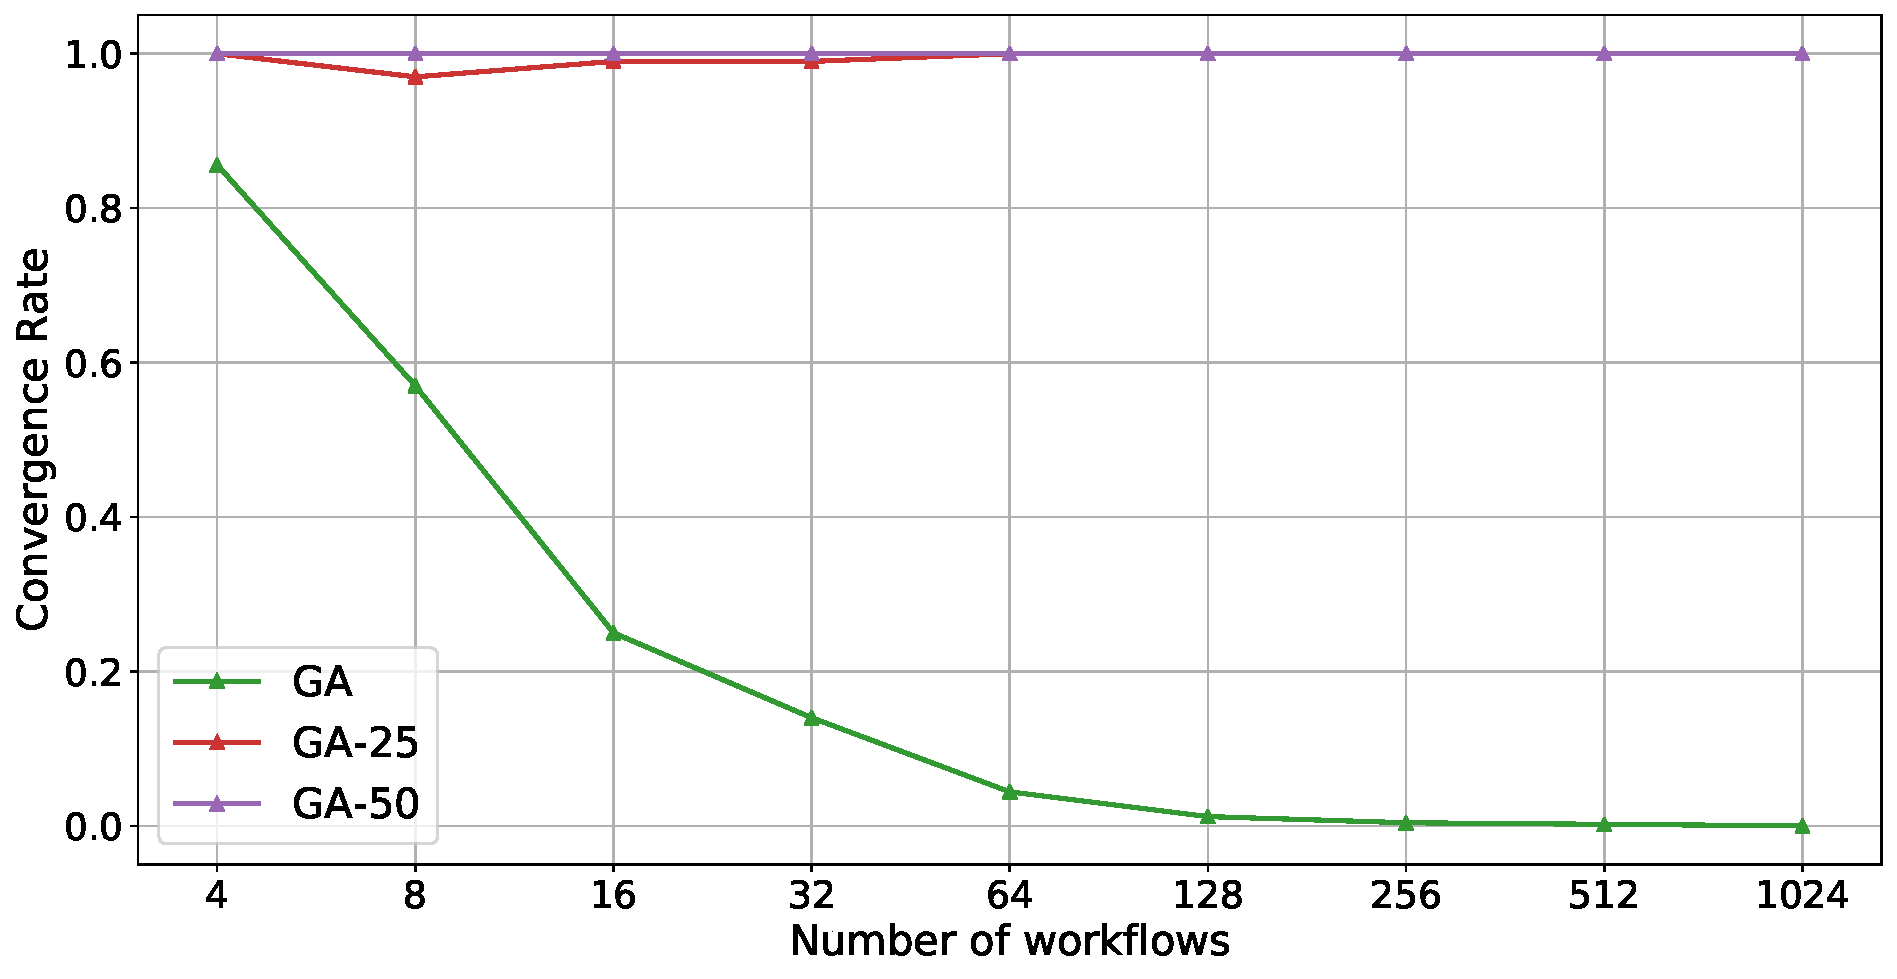
\includegraphics[width=.95\textwidth]{figures/campaign/StHomoCampaigns_4StHomoResourcesGAconv.pdf}
        \caption{}
        \label{fig:ga_conv1}
    \end{subfigure}\\
    ~ 
    \begin{subfigure}[b]{0.75\textwidth}
        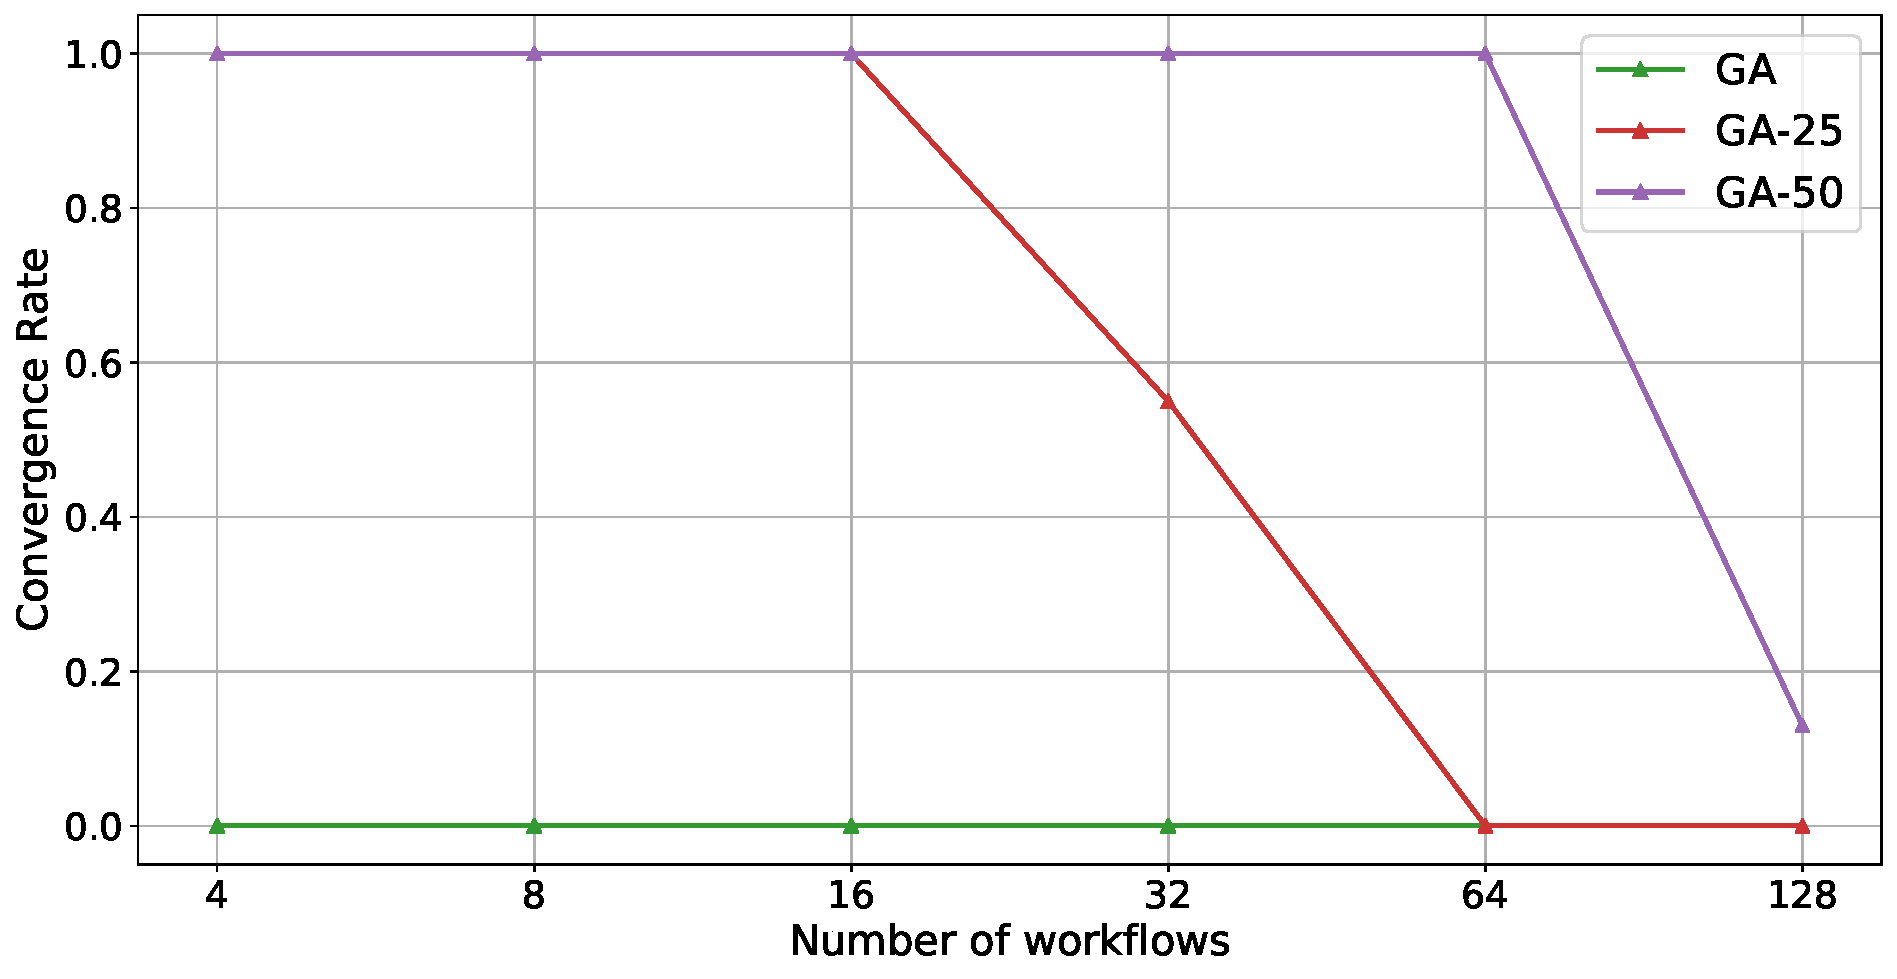
\includegraphics[width=.95\textwidth]{figures/campaign/HomogeResources_StHomogeCampaignsGAconv.pdf}
        \caption{}
        \label{fig:ga_conv2}
    \end{subfigure}
    \caption{Convergence rate of Genetic algorithm for homogeneous campaigns on static homogeneous resources based on random initialization percentage: ~\ref{fig:ga_conv1}) Different campaign sizes on 4 resources;~\ref{fig:ga_conv2}) Campaign with 1024 workflows and different number of resources.}
    \label{fig:conv_rate}
\end{figure*}

Figure~\ref{fig:ga_conv2} shows the convergence rate of the genetic algorithm as the number of resources changes while the number of workflows is constant.
When the population is initialized randomly, the genetic algorithm does not produce a plan that has the ideal makespan.
The convergence rate of GA-25 is 1 up to 16 resource and drops to 0 for more than 32 resources.
GA-50 convergence rate is 1 up to 64 resources and drops to less than 0.2 for 128 resources and equal to 0 for 256 resources.
The drop is due to the random initial placement of workflows on resources.
As the number of resources increase, the probability for GA to place less than $ N_{C} \ N_{R} $ workflows on a resource decreases.

Based the convergence rate, we expect that GA will not provide on average a plan with the ideal makespan whether the campaign size changes or the number of resources.
GA-25 will provide plans with the ideal makespan when the number of resources is less than 16 regardless the number of workflows.
Finally, GA-50 will provide plans with ideal makespan up to 64 resources.

Figure~\ref{fig:st_homog_analysis} shows the makespan for a campaign with homogeneous workflows and homogeneous resources a plan which uses HEFT, GA (for the three different configurations), L2FF and random (RA).
Figure~\ref{fig:StHomoCampaigns_4StHomoResources} varies the campaign size from 4 to 2048 workflows while the number of resources is equal to 4 and figure~\ref{fig:StHomoResources_StHomoCampaigns} varies the number of resources from 4 to 256 resources while the campaign size equals to 1024 workflows.

\begin{figure}[ht!]
    \centering
    \begin{subfigure}[b]{0.75\textwidth}
        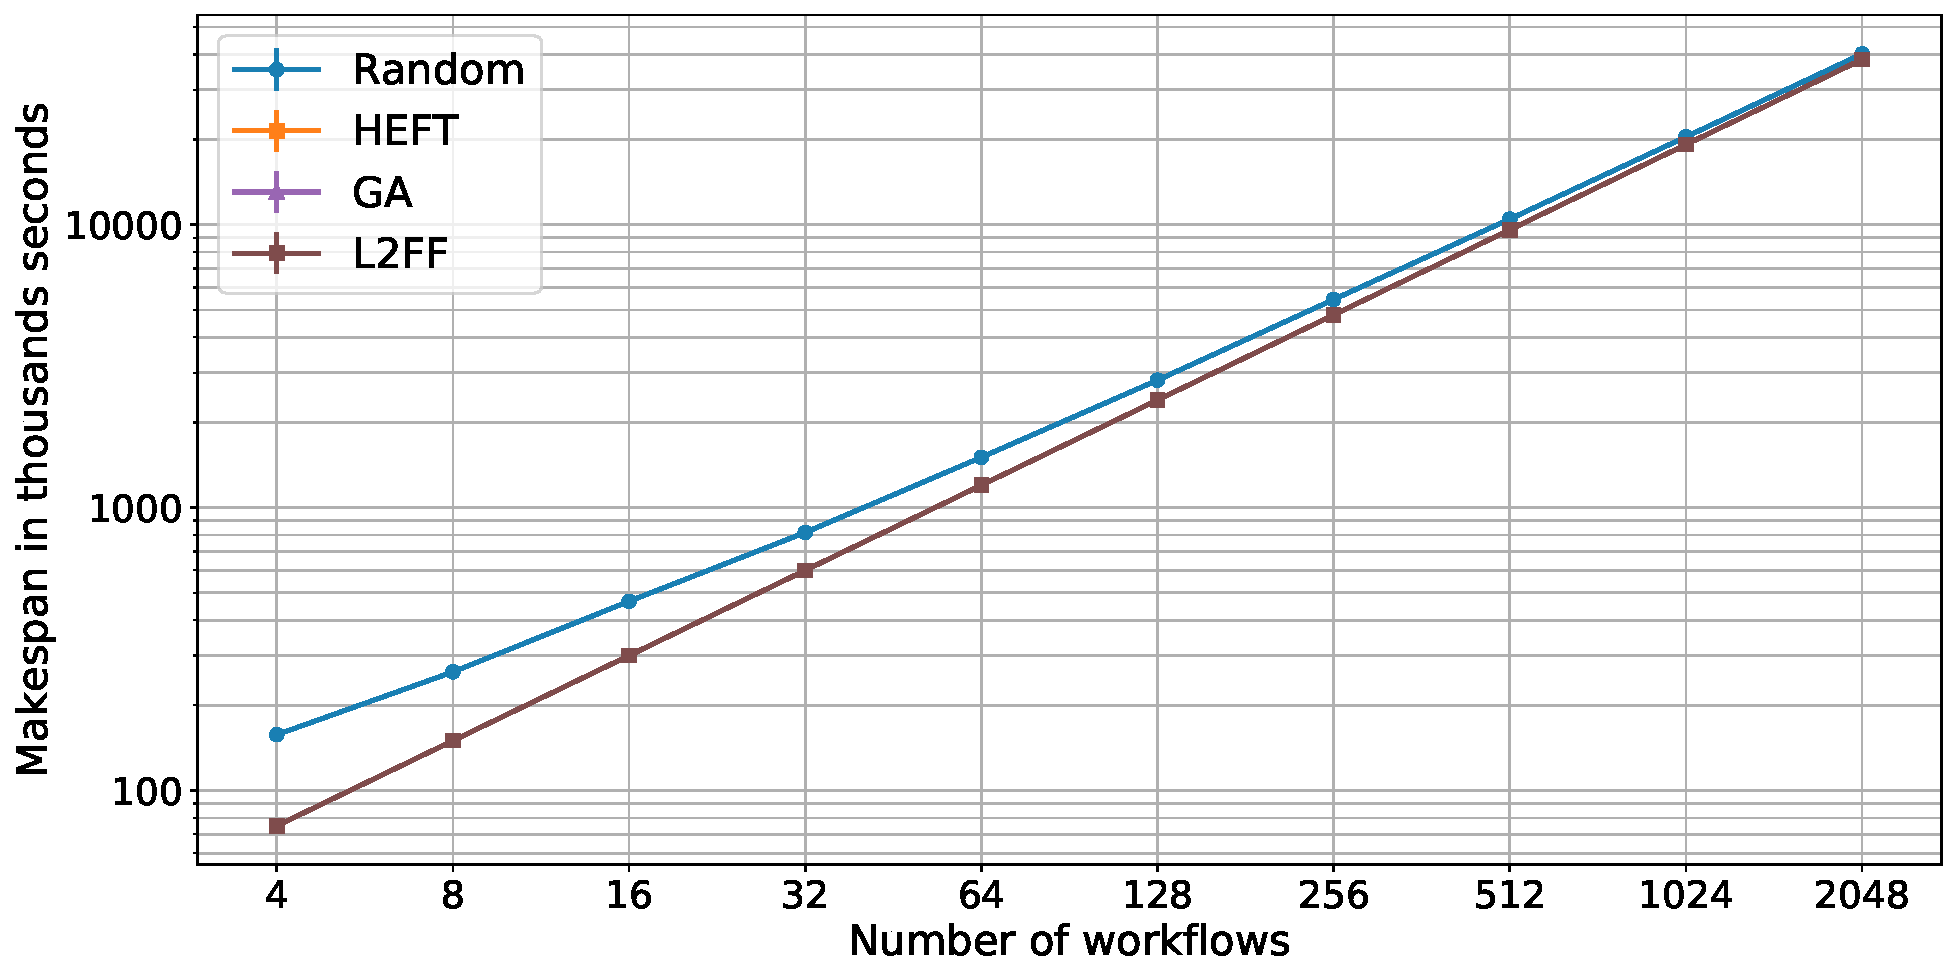
\includegraphics[width=.95\textwidth]{figures/campaign/StHomoCampaigns_4StHomoResources.pdf}
        \caption{}
        \label{fig:StHomoCampaigns_4StHomoResources}
    \end{subfigure}\\
    ~ 
    \begin{subfigure}[b]{0.75\textwidth}
        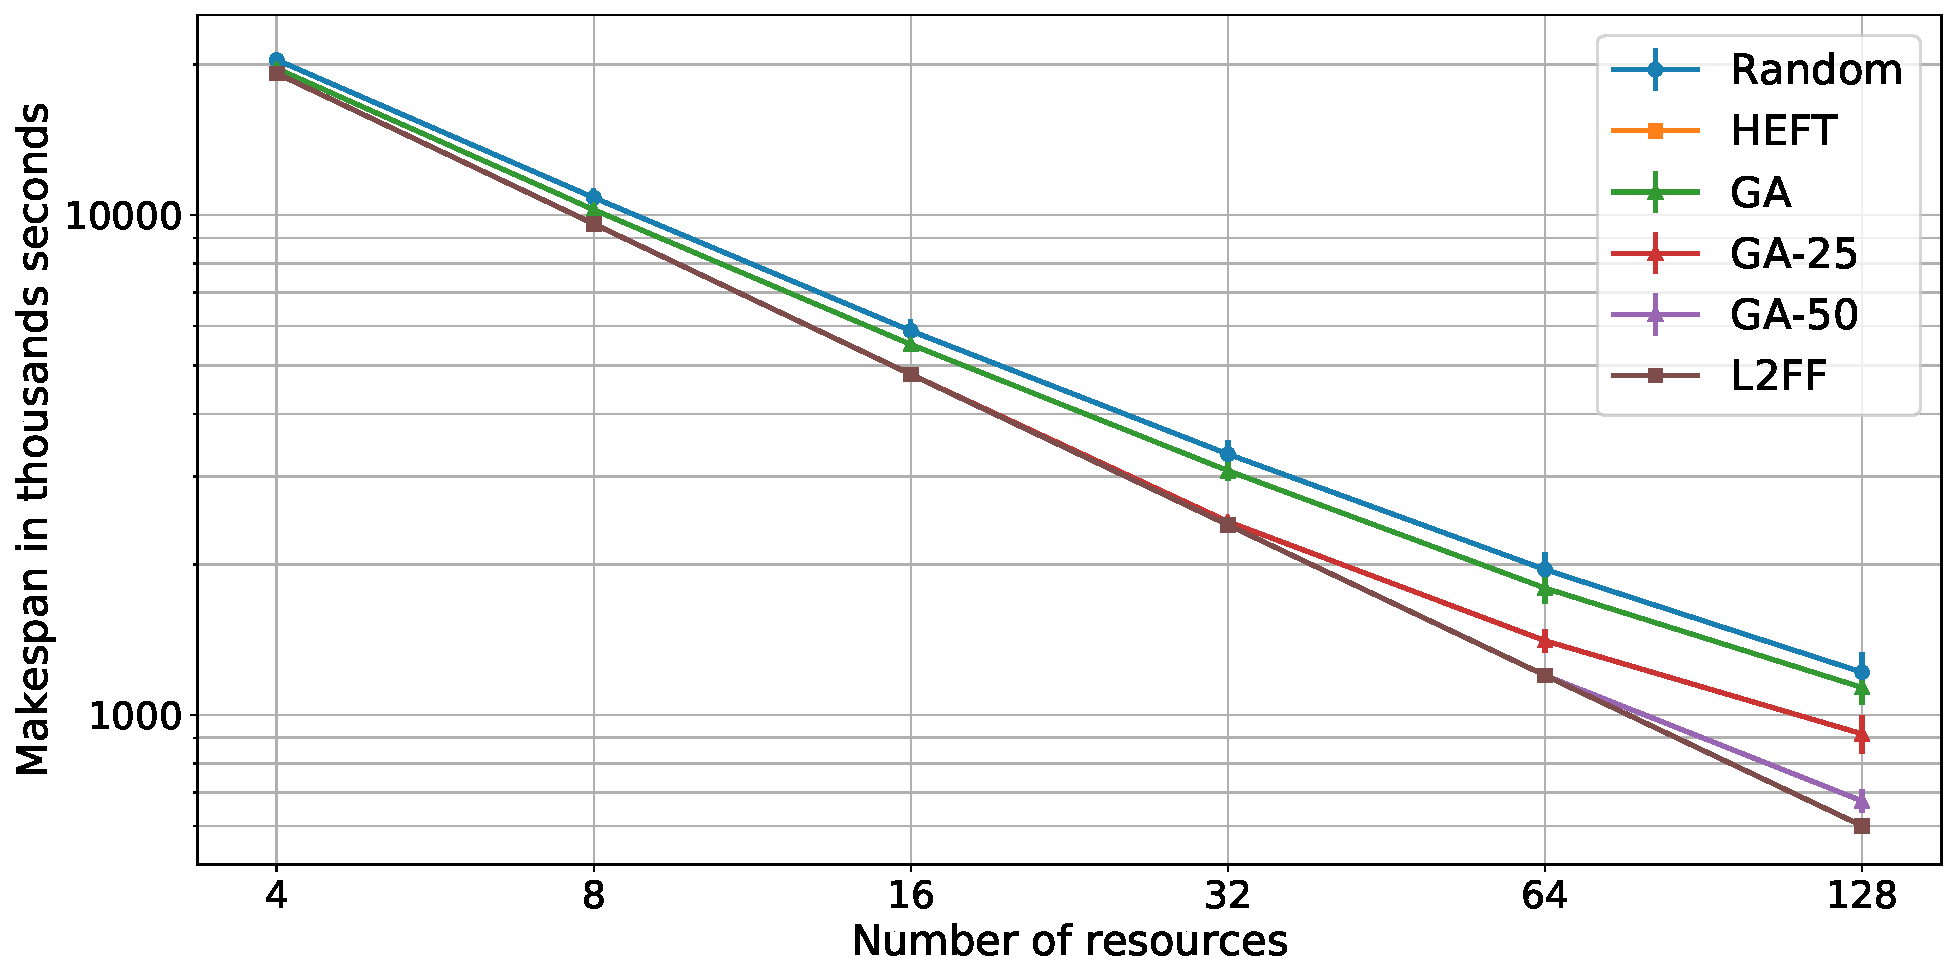
\includegraphics[width=.95\textwidth]{figures/campaign/StHomoResources_StHomoCampaigns.pdf}
        \caption{}
        \label{fig:StHomoResources_StHomoCampaigns}
    \end{subfigure}
    \caption{~\ref{fig:StHomoCampaigns_4StHomoResources} Makespan of increasing number of homogeneous workflows on homogeneous resources.
    ~\ref{fig:StHomoResources_StHomoCampaigns} Makespan of homogeneous campaign on different number of homogeneous resources.}
    \label{fig:st_homog_analysis}
\end{figure}

HEFT and L2FF provide better makespan that Random and the genetic algorithm.
L2FF places equal number of workflows per resource for all available resources.
HEFT places a workflow to the resource that will finish it earlier.
This in turn means that it will place a workflow on the resource that has less workflows that any other resource.
As a result, both algorithms are able to equally distribute the workflows to the resources.

The genetic algorithm makespan performance confirms our expectation providing different makespans based on the percentage of workflows that are assigned non-randomly.
Although all three configurations produce plans with small differences when the number of workflows changes, GA produces plans that are very close to random as the number of resources increase, less than 8~\% difference.
GA-25 and GA-50 produce plans with up to 25~\% and 50~\% better performance than random respectively.
In addition as expected by the convergence rate values, start to produce plans different than HEFT and L2FF over 16 and 64 resources respectively.
As GA-50 provides plans with the best makespan over the three different configurations, we will show only GA-50 from now on.

The next configuration of this experiment shows how resource heterogeneity affects the performance of the algorithms.
All algorithms produce and use different information about resources and specifically resource availability.
Based on the information they produce, we expect the algorithms that produce more exact information to have better performance, such as HEFT and GA-50.

\begin{figure*}[ht!]
    \centering
    \begin{subfigure}[b]{0.75\textwidth}
        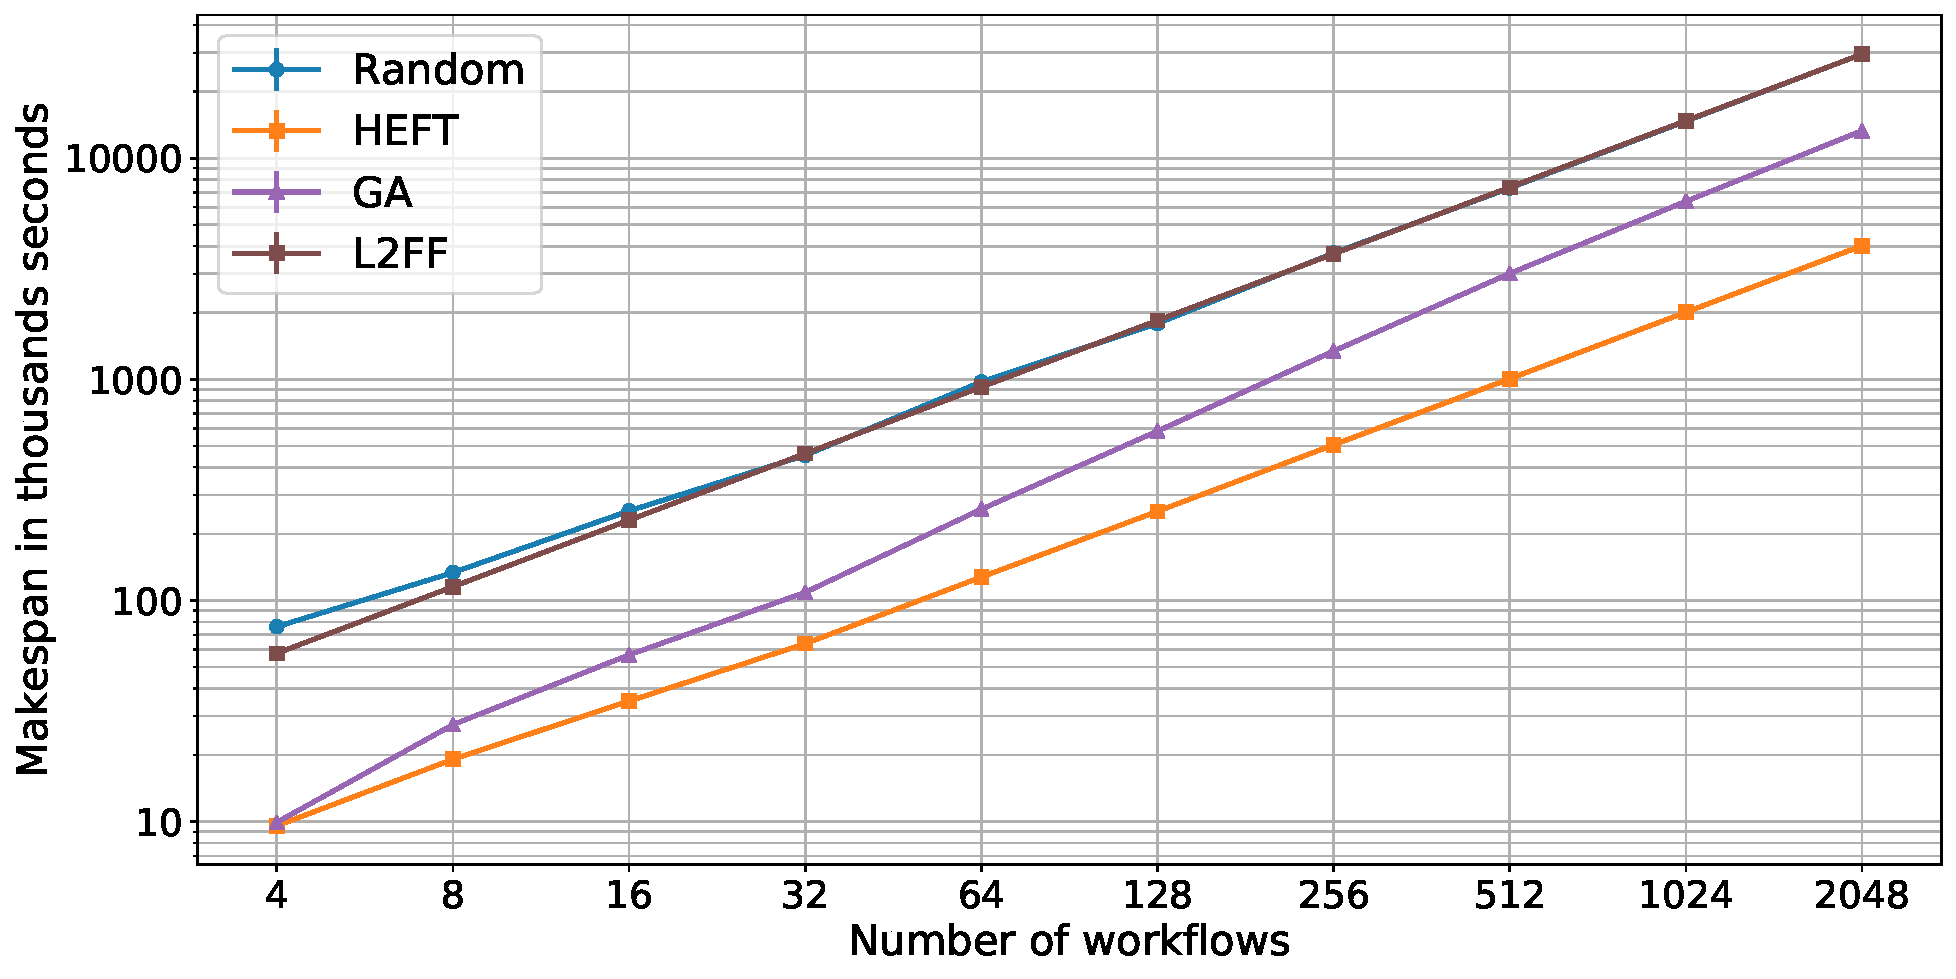
\includegraphics[width=.95\textwidth]{figures/campaign/StHomoCampaigns_4StHeteroResources.pdf}
        \caption{}
        \label{fig:StHomoCampaigns_4StHeteroResources}
    \end{subfigure}\\
    ~ 
    \begin{subfigure}[b]{0.75\textwidth}
        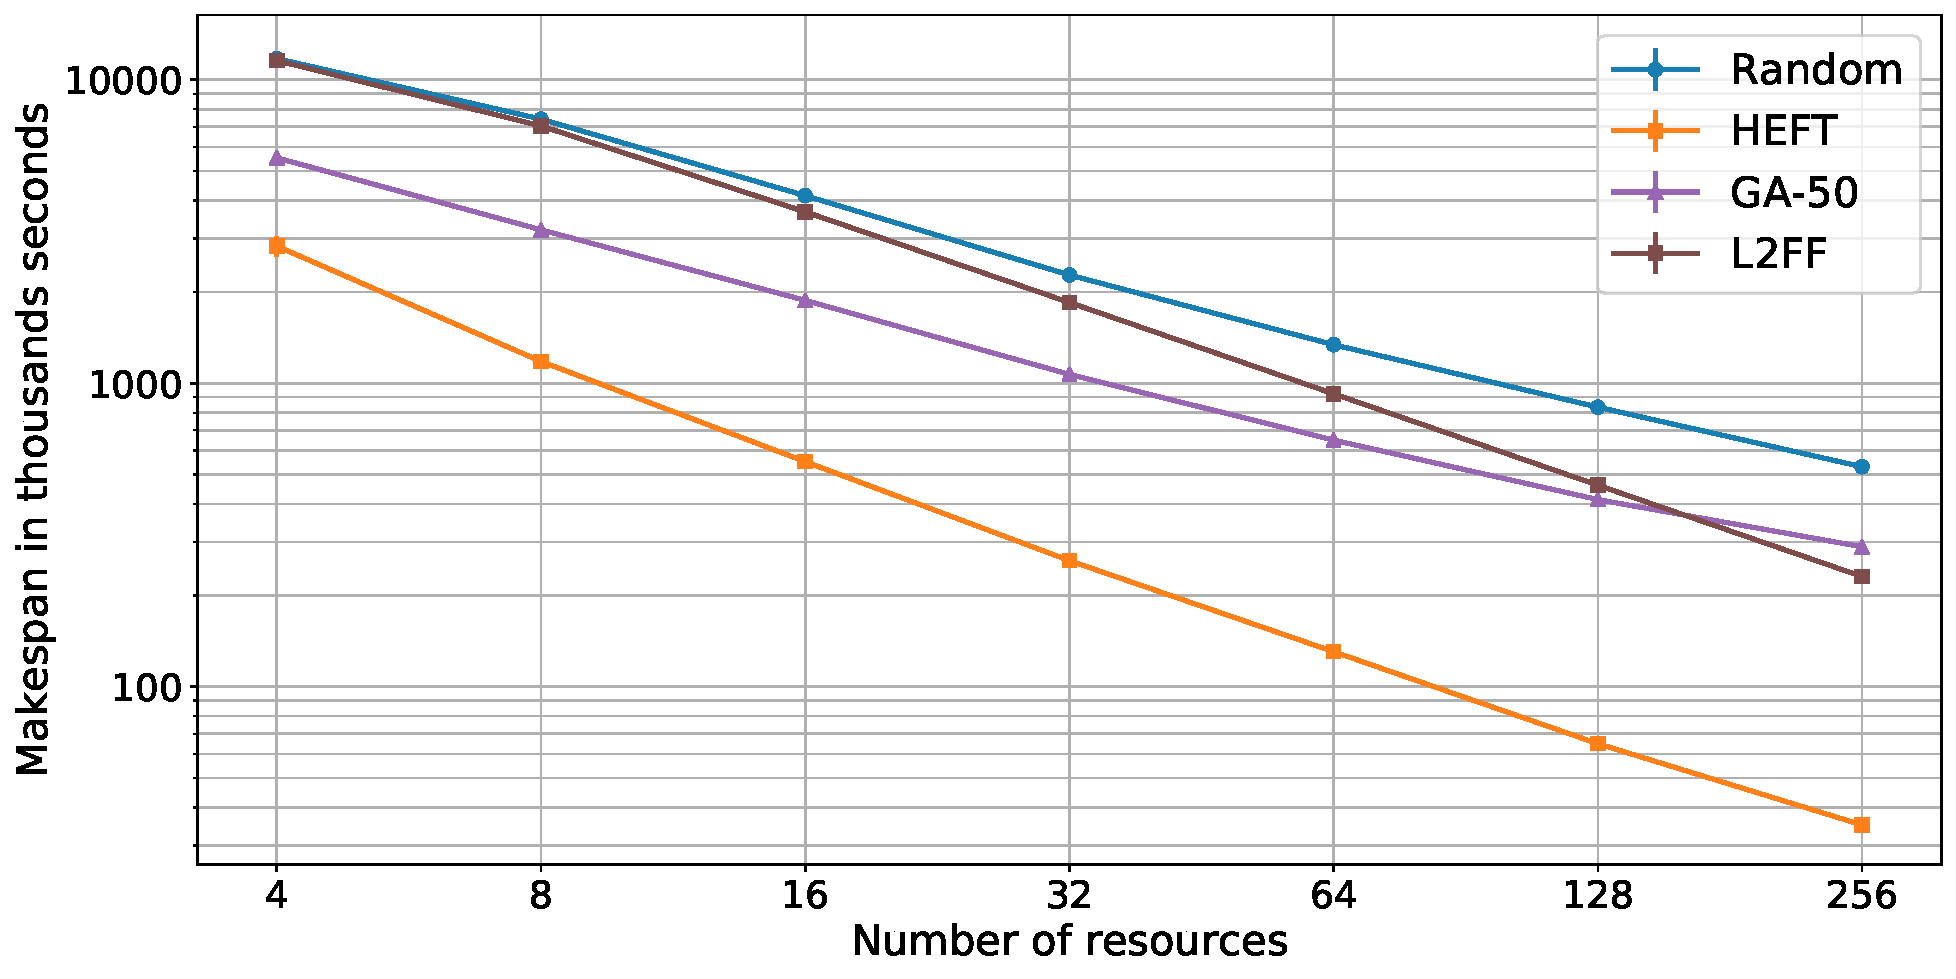
\includegraphics[width=.95\textwidth]{figures/campaign/StHeteroResources_StHomoCampaigns.pdf}
        \caption{}
        \label{fig:HeteroResources_StHomoCampaigns}
    \end{subfigure}
    \caption{Makespan of homogeneous worklfows on heterogeneous resources:~\ref{fig:StHomoCampaigns_4StHeteroResources}) varying campaign size with 4 resources;
        ~\ref{fig:HeteroResources_StHomoCampaigns}) varying number of resources for constant campaign size at 1024 workflows.}
    \label{fig:hom_het_analysis}
\end{figure*}

Figure~\ref{fig:hom_het_analysis} shows the makespan of the three algorithms for a campaign with homogeneous workflows on heterogeneous resources.
HEFT provides up to an order of magnitude better makespan than L2FF and GA-50 whether the campaign size changes (Fig.~\ref{fig:StHomoCampaigns_4StHeteroResources}) or the number of resources (Fig.~\ref{fig:HeteroResources_StHomoCampaigns}).
In addition, GA-50 produces plans with at least two times better makespan that L2FF when resources are constant and the number of workflows changes.
As the number of resources increase, the difference between the plans that GA-50 and L2FF produce reduces with L2FF providing a plan with better makespan than GA-50 for 256 resources.
Due to the partial random initialization of  its plans, the genetic algorithm under-utilize some resources and over utilizes others.
Instead, L2FF places the same number of workflows per resource and as a result overutilizes less performant resources.
%This leads to the believe that GA-50 places more than 8 and 4 workflows on the less performant resources for 128 and 256 resources respectively.
Further, HEFT is ranking the workflows and also places a workflow to the resource that will finish it earlier.
As a result, HEFT utilizes resources so that for every placement the makespan increase is the least possible.


\begin{figure*}[ht!]
    \centering
    \begin{subfigure}[b]{0.75\textwidth}
        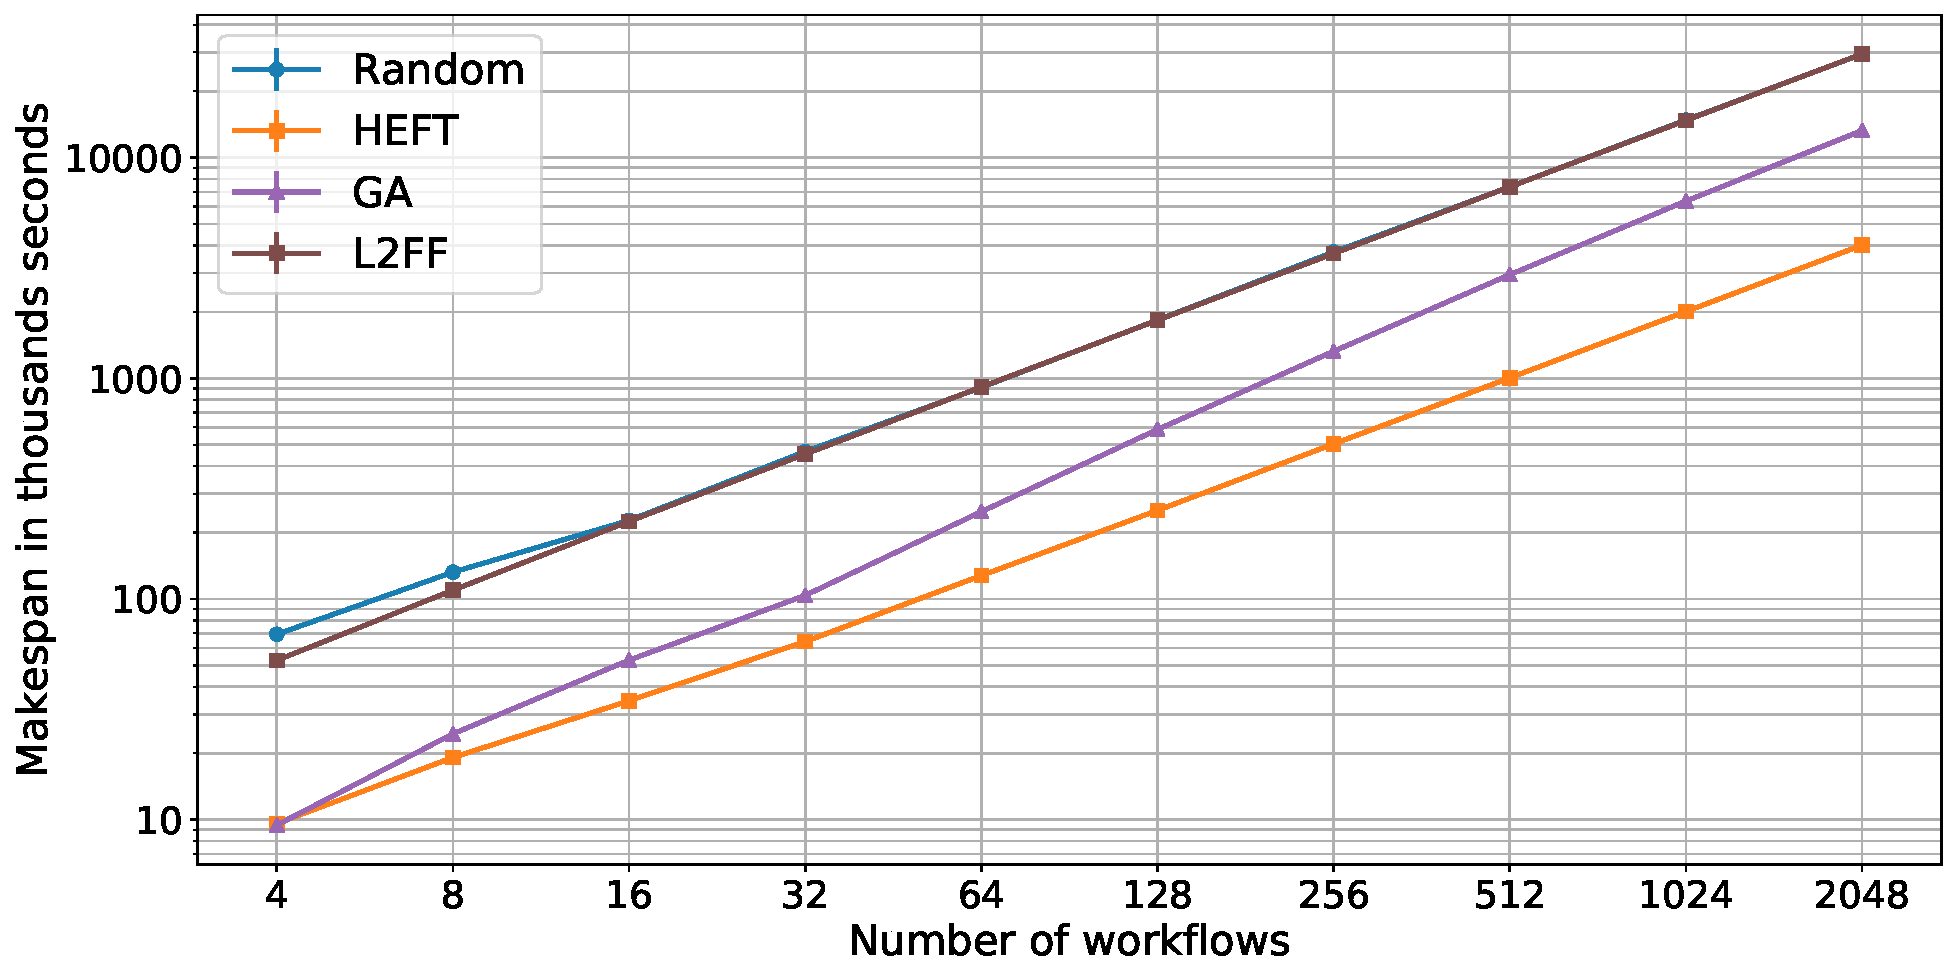
\includegraphics[width=.95\textwidth]{figures/campaign/StHeteroCampaigns_4StHeteroResources.pdf}
        \caption{}
        \label{fig:StHeteroCampaigns_4StHeteroResources}
    \end{subfigure}\\
    ~ 
    \begin{subfigure}[b]{0.75\textwidth}
        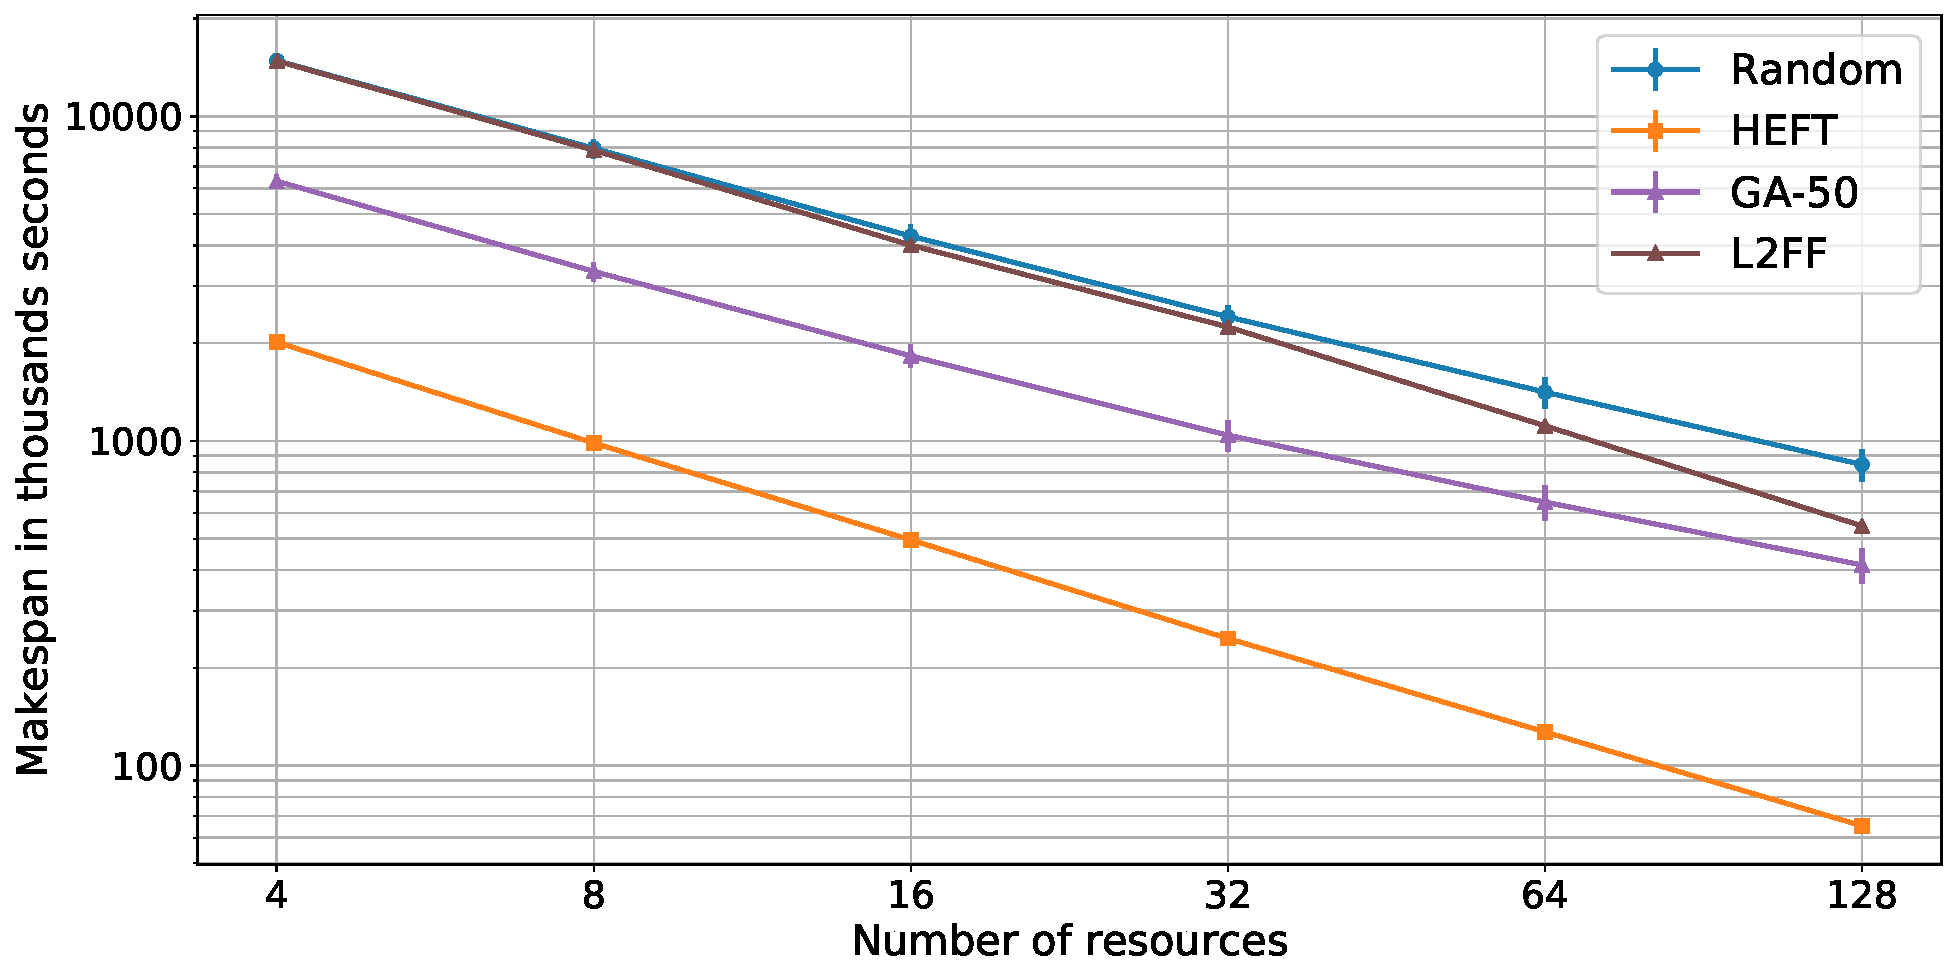
\includegraphics[width=.95\textwidth]{figures/campaign/StHeteroResources_StHeteroCampaigns.pdf}
        \caption{}
        \label{fig:StHeteroResources_StHeteroCampaigns}
    \end{subfigure}
    \caption{~\ref{fig:StHeteroCampaigns_4StHeteroResources}) Makespan of increasing number of heterogeneous workflows on heterogeneous resources;
        ~\ref{fig:StHeteroResources_StHeteroCampaigns}) Makespan of heterogeneous campaign on different number of heterogeneous resources.}
    \label{fig:heter_analysis}
\end{figure*}

Figure~\ref{fig:heter_analysis} shows the performance of the algorithms when a campaign with heterogeneous workflows executes on heterogeneous resources.
Comparing the results with those in figure~\ref{fig:hom_het_analysis}, there is not significant difference in the performance of the algorithms due to workflow heterogeneity from our use case.
This leads to the conclusion that resource heterogeneity affects the performance of the algorithms more than workflow heterogeneity.

In summary, we can conclude that resource heterogeneity dominates the makespan performance among the considered algorithms.
On homogeneous resources, HEFT, GA-50 and L2FF plans produce plans with similar makespan.
On heterogeneous resources, HEFT makespan is at least an order of magnitude smaller than L2FF makespan and is more than two times smaller than GA-50 makespan independent of workflow homogeneity or heterogeneity.
Based on our analysis, the characteristics of the selected algorithms that affect the makespan performance are:
\begin{inparaenum}[1)]
    \item estimating when a resource will be available;
    \item deterministic or randomized heuristics; and
    \item creating a workflow priority list based on workflow runtime
\end{inparaenum}

\subsection{Experiment 2: Sensitivity of makespan to resource dynamism}

High performance computing (HPC) resources show performance variations for multiple reasons, including power constrained operations~\cite{inadomi2015analyzing}, network and shared filesystem congestion~\cite{brown2018interference} and performance degradation~\cite{wu2017survey}.
In addition, the timescales of the variations span from day to years~\cite{skinner2005understanding}.
We model resource dynamism as a normal distribution with a mean value equal to the performance of a resource and sigma to 6~\% of the mean, resulting to $\pm$ 20~\% change in resource performance.
Further, we assume that the performance changes daily and as a result affects the execution of the workflows of the selected use case.
Figure~\ref{fig:dynamic_res} shows a histogram of a dynamic resource performance with a mean value equal to 1 petaFLOP.

\begin{figure}[t]
    \centering
    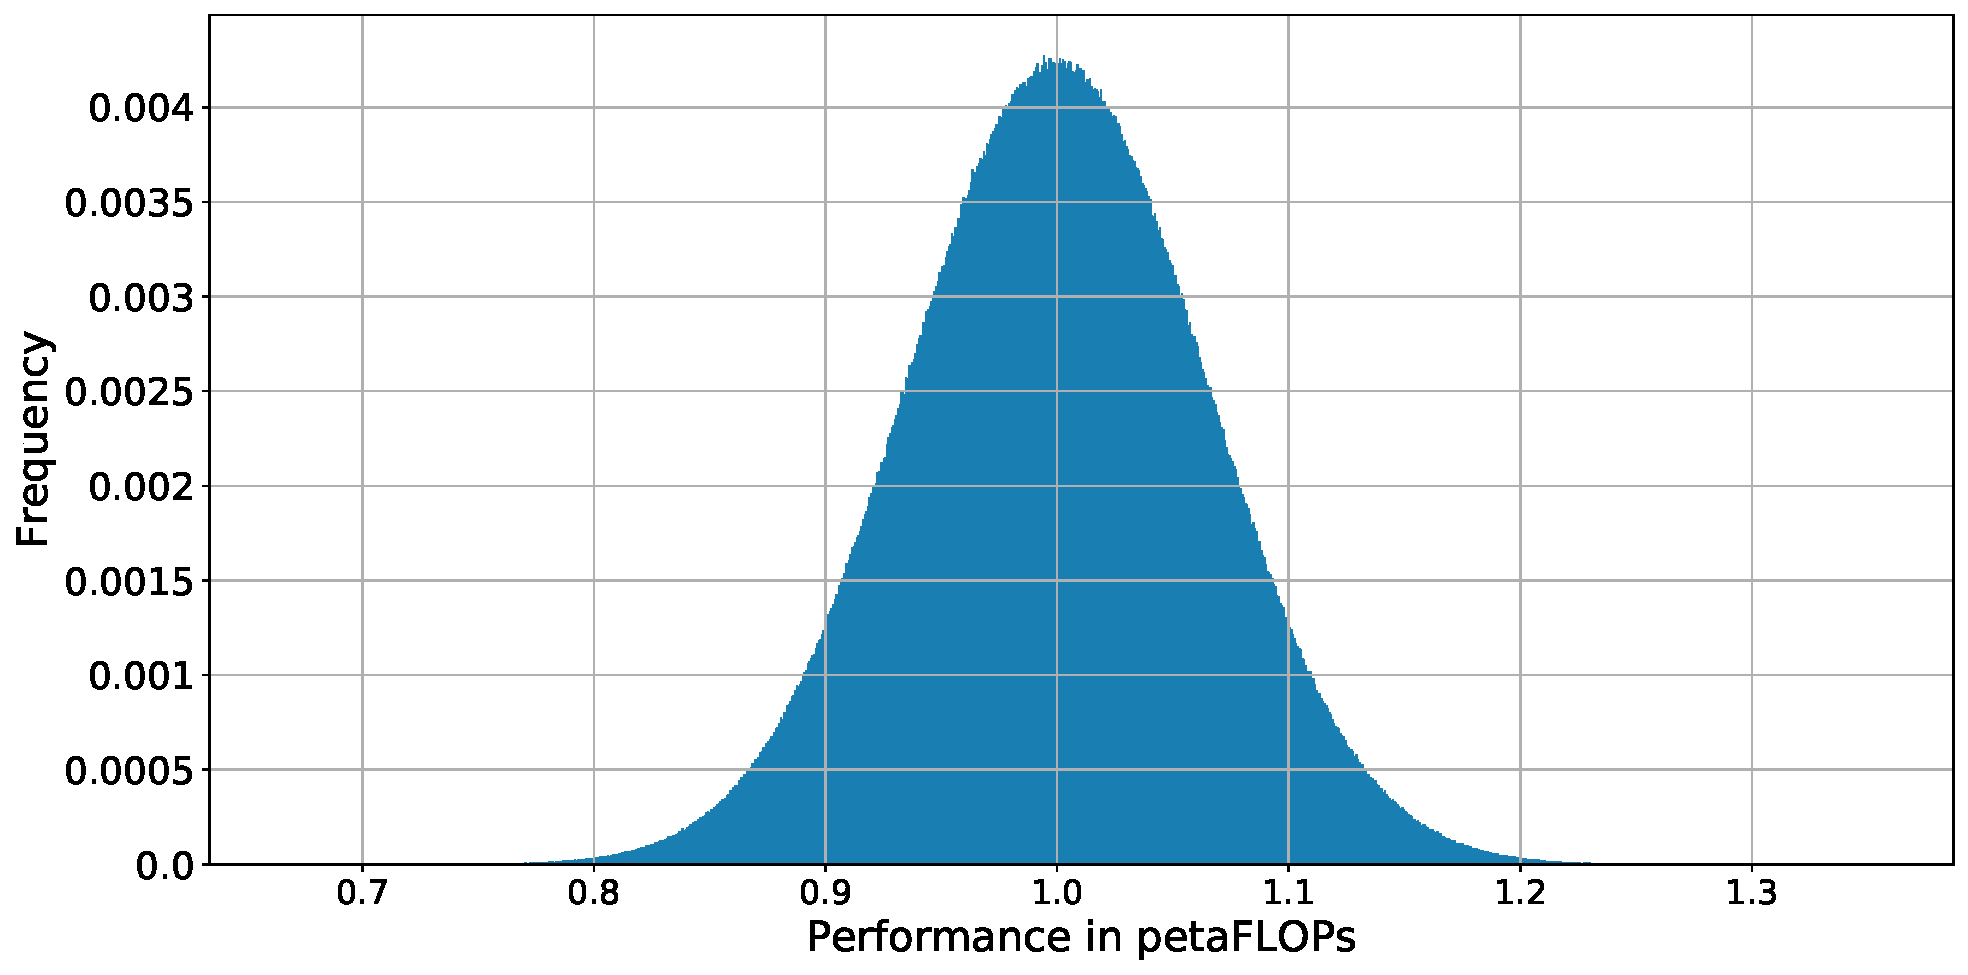
\includegraphics[width=.75\textwidth]{figures/campaign/DynRes.pdf}
    \caption{Resource performance distribution of a dynamic resource with 1 petaFLOP average performance.}
    \label{fig:dynamic_res}
\end{figure}

In this experiment, we measure the sensitivity of the makespan using HEFT, L2FF, GA-50 and Random on homogeneous and heterogeneous resources.
We define as makespan sensitivity the difference between the makespan measured via executing a campaign and the expected makespan given by the execution plan.
In addition, all workflows are assigned to a resource before executing the campaign and that assignment does not change during runtime.
Based on our understanding from experiment 1, we expect the sensitivity to be similar between algorithms on homogeneous resources, as all three algorithms produce similar plans.
Figures~\ref{fig:dyn_homog_sens_analysis} and~\ref{fig:dyn_hetero_sens_analysis} show the results for homogeneous workflows/ homogeneous resources and heterogeneous workflows/ heterogeneous resources respectively.

As per our expectation, the sensitivity of makespan among the three algorithms is similar and it is between 1~\% and 10~\% (see Fig.~\ref{fig:StHomoCampaigns_4DyHomoResourcesSens} and~\ref{fig:DyHomoResources_StHomoCampaignsSens}).
In addition, we observe a drop in GA-50 sensitivity at 128 resources.
This is because, GA-50 produces different plans at every realization of the experiment, since it places a number of workflows to resources randomly.
In addition, the sensitivity drops as the number of workflows increase and the number of resources is constant ( Fig.~\ref{fig:StHomoCampaigns_4DyHomoResourcesSens}) and increases when the number of resources increase and the number of workflows is constant (Fig.~\ref{fig:DyHomoResources_StHomoCampaignsSens}).
Thus, as the average number of workflows per resource increases the sensitivity decreases regardless how workflows are placed onto resource by a plan.


\begin{figure}[ht!]
    \centering
    \begin{subfigure}[b]{0.75\textwidth}
        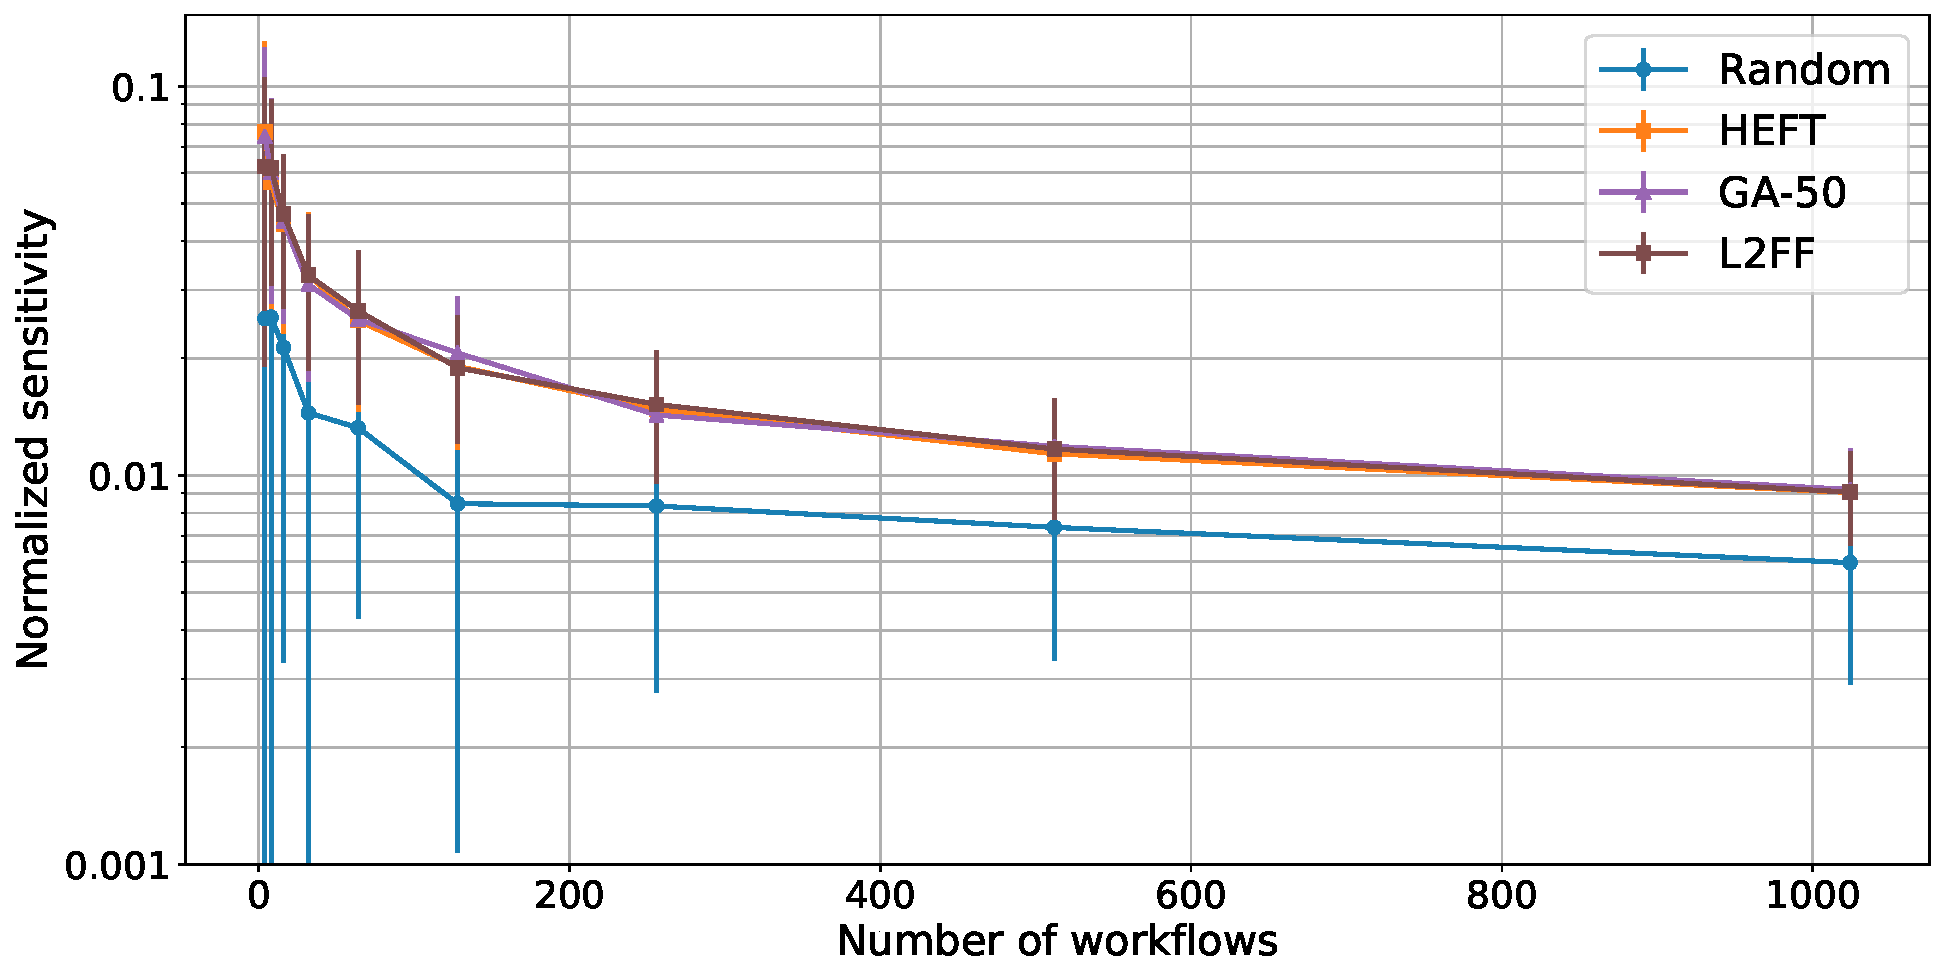
\includegraphics[width=.95\textwidth]{figures/campaign/StHomoCampaigns_4DynHomoResourcesSens.pdf}
        \caption{}
        \label{fig:StHomoCampaigns_4DyHomoResourcesSens}
    \end{subfigure}\\
    ~ 
    \begin{subfigure}[b]{0.75\textwidth}
        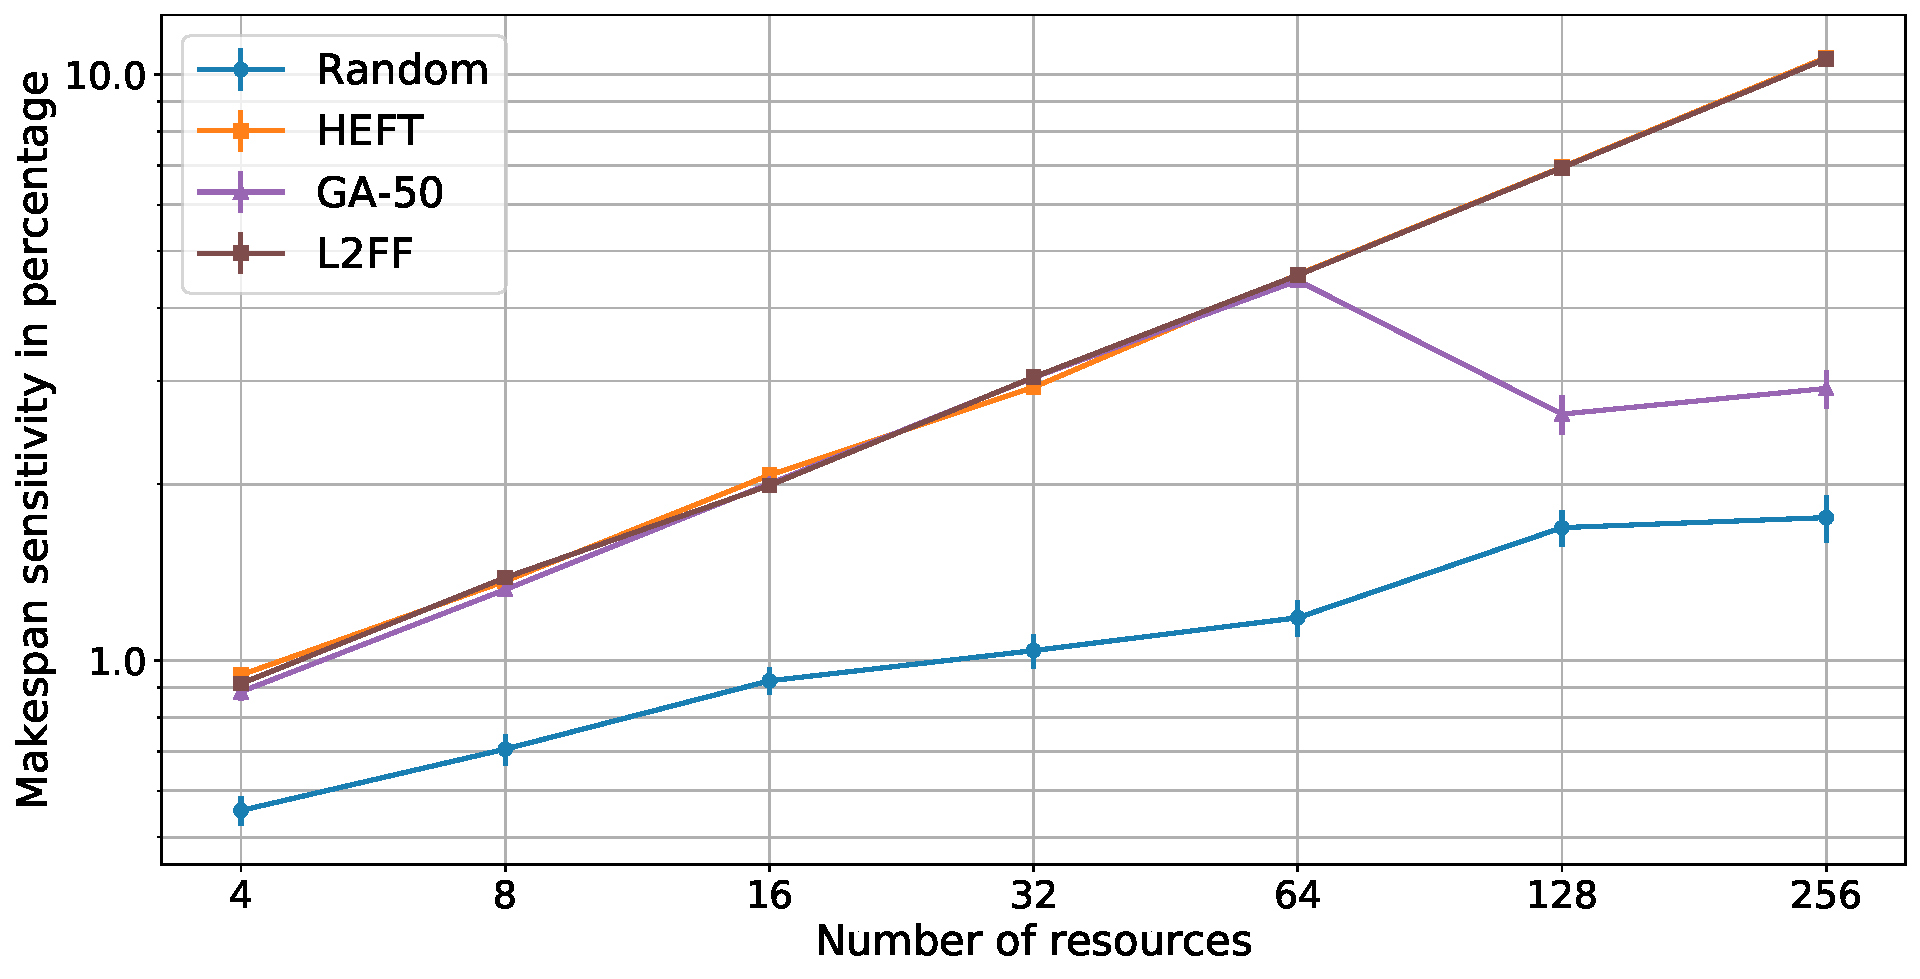
\includegraphics[width=0.95\textwidth]{figures/campaign/DynHomoResources_StHomoCampaignsSens.pdf}
        \caption{}
        \label{fig:DyHomoResources_StHomoCampaignsSens}
    \end{subfigure}
    \caption{Sensitivity of makespan in percentage of homogeneous workflows on homogeneous resources for:~\ref{fig:StHomoCampaigns_4DyHomoResourcesSens} increasing number of workflows and 4 resources;
        ~\ref{fig:DyHomoResources_StHomoCampaignsSens} on increasing number of resources and 1024 workflows.}
    \label{fig:dyn_homog_sens_analysis}
\end{figure}


Figure~\ref{fig:dyn_hetero_sens_analysis} shows the makespan sensitivity as a percentage for a campaign of heterogeneous workflows and heterogeneous resources.
We excluded the case of homogeneous workflows as it is similar in terms of makespan to executing heterogeneous workflows on heterogeneous resources.
Based on the two subplots, we see that sensitivity decreases as the number of workflows increase and increase as the number of resources increase.
This further supports our conclusion that as the average number of workflows per resource increases the sensitivity decreases.
Makespan sensitivity shows similar values for all three algorithms in figure~\ref{fig:StHeteroCampaigns_4DyHeteroResourcesSens}, except HEFT for more than 512 workflows.
HEFT places workflows on resources in such a way that each resource will be used for similar amount of time.
As a result, a slow down on a resource will affect the makespan more than GA-50 and L2FF which produce plans that overutilize some resources.

Based on the results in figure~\ref{fig:DyHeteroResources_StHeteroCampaignsSens} we see that the number of resources is a more dominant factor than resource heterogeneity for makespan sensitivity.
HEFT-based plan is more sensitive that GA-50, L2FF and Random up to 64 resources.
L2FF becomes more sensitive for more than 128 resources and is more sensitive to changes on less performant resources.

\begin{figure}[ht!]
    \centering
    \begin{subfigure}[b]{0.85\textwidth}
        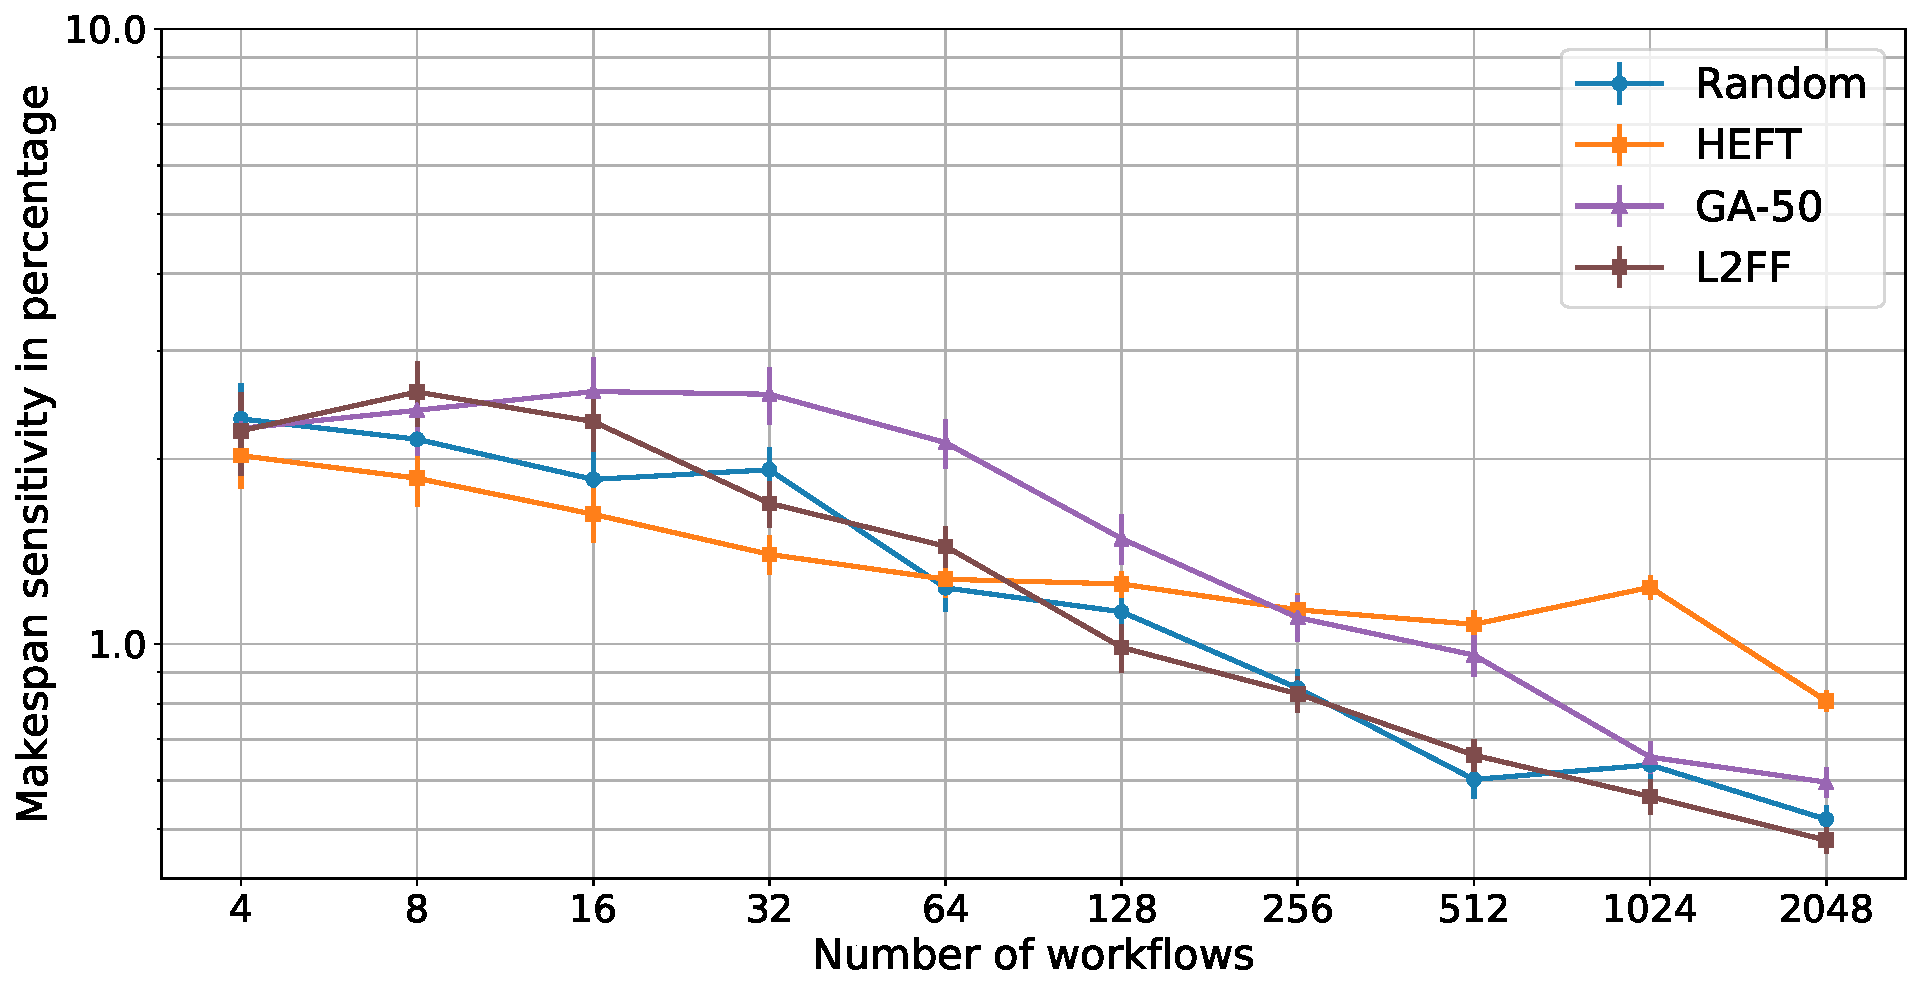
\includegraphics[width=.95\textwidth]{figures/campaign/StHeteroCampaigns_4DynHeteroResourcesSens.pdf}
        \caption{}
        \label{fig:StHeteroCampaigns_4DyHeteroResourcesSens}
    \end{subfigure}\\
    ~ 
    \begin{subfigure}[b]{0.85\textwidth}
        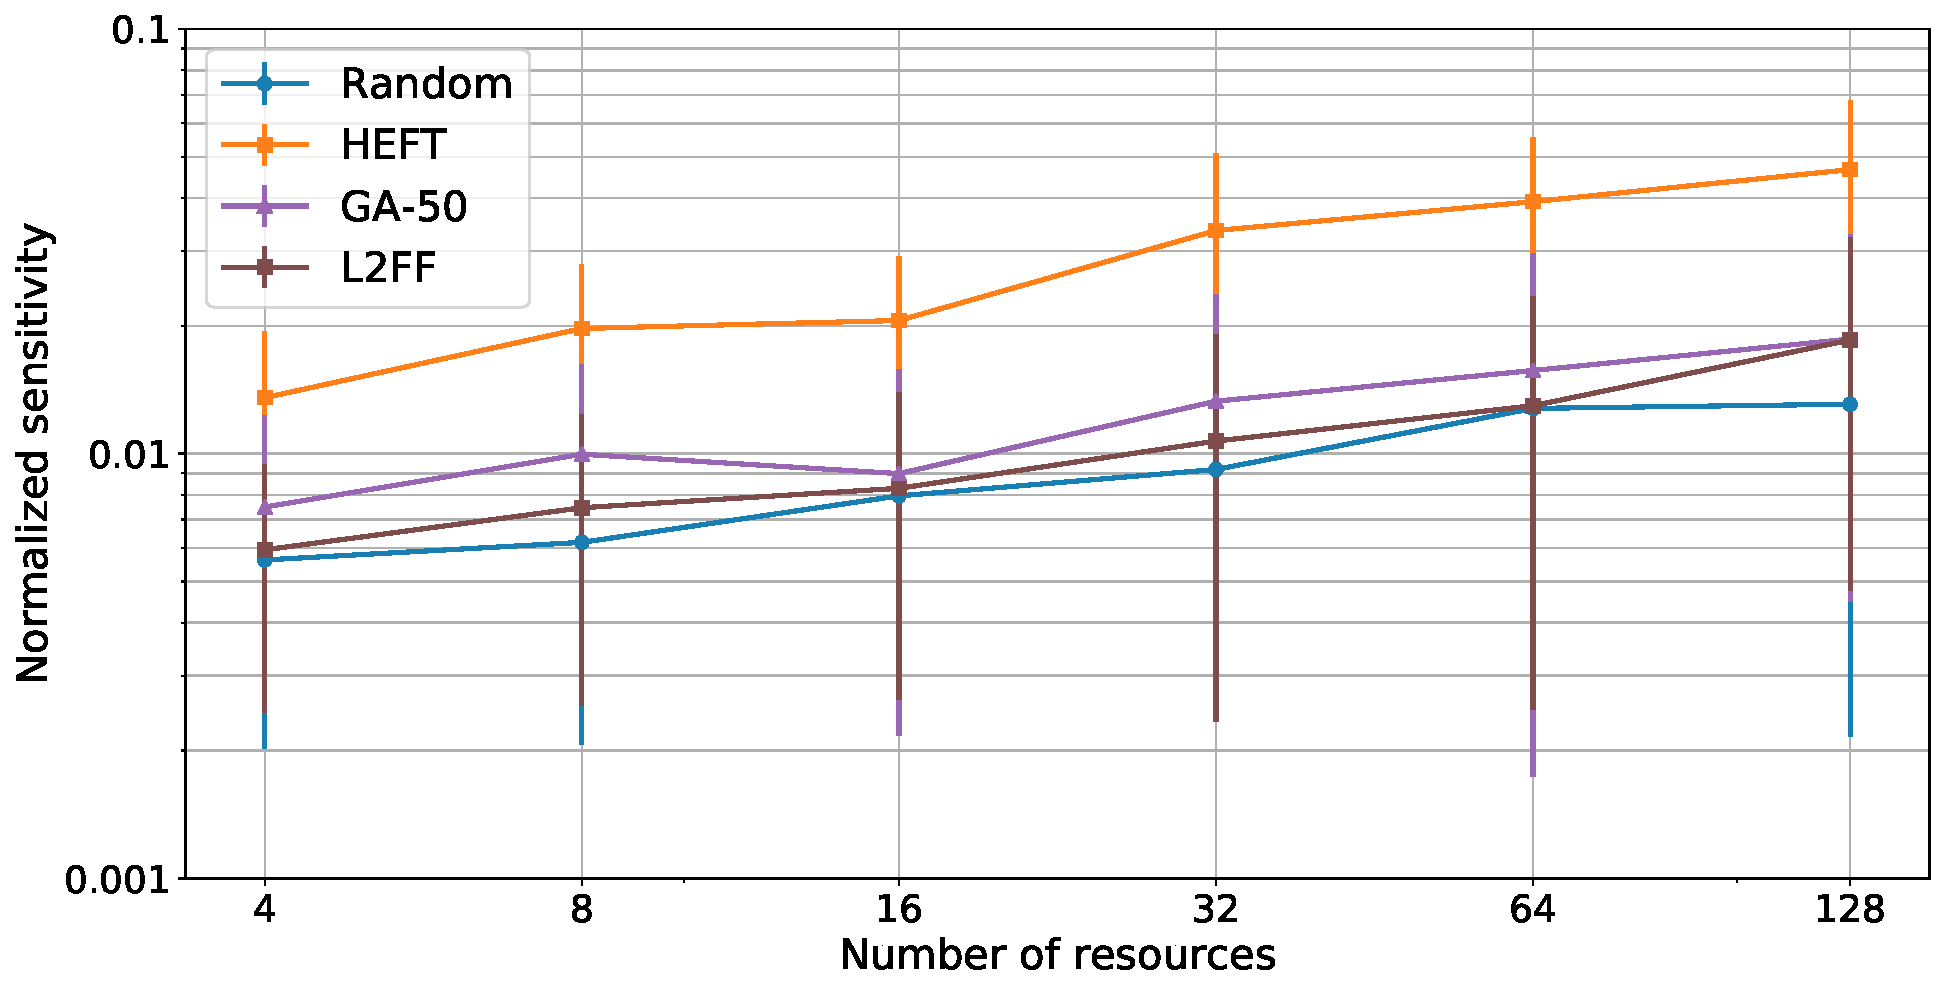
\includegraphics[width=0.95\textwidth]{figures/campaign/DynHeteroResources_StHeteroCampaignsSens.pdf}
        \caption{}
        \label{fig:DyHeteroResources_StHeteroCampaignsSens}
    \end{subfigure}
    \caption{Sensitivity of makespan in percentage of heterogeneous workflows on heterogeneous resources for:~\ref{fig:StHeteroCampaigns_4DyHeteroResourcesSens}  increasing number of workflows and 4 resources; and
    ~\ref{fig:DyHeteroResources_StHeteroCampaignsSens} on increasing number of resources and 1024 workflows.}
    \label{fig:dyn_hetero_sens_analysis}
\end{figure}

This experiment measured how sensitive are plans using HEFT, GA, L2FF and Random to resource dynamism.
On homogeneous resources, all algorithms show similar levels of sensitivity.
GA-50 sensitivity drops from more than 64 resources as some resources are overutilized.
On heterogeneous resources, HEFT is generally more sensitive since it uses an expectation about resource availability to map workflows to resources.
L2FF becomes more sensitive than HEFT after 128 resources as it places equal number of workflows to resources overutilizing less performant resources.
In addition, sensitivity is proportional to the number of resources and inverse proportional to the number of workflows, since it decreases as the number of workflows increase when using constant number of resources and increases when number of resources increases and campaign size is constant.
Finally, we observed that for a 6~\% temporal resource variation causes less than 10~\% variation in makespan regardless if resources are homogeneous or heterogeneous.


\subsection{Experiment 3: Sensitivity of makespan to workflow runtime estimation uncertainty}

All of the selected algorithms require an estimation about the runtime of each workflow of the campaign.
Users usually offer this kind of information as a range of values drawn by empirical data.
As a result, there is a level of uncertainty in the workflow runtime estimation.
This experiment measures how sensitive are the plans produced by the selected algorithms for different levels of uncertainty.

We introduce workflow runtime estimation uncertainty as the difference between the estimated and actual runtime of a workflow on a 1 petaFLOP resource.
Specifically, we denote as $u$ the level of uncertainty between $[0,1)$, $u'$ the uncertainty for a workflow drawn randomly from the range $[-u,u]$ and $Tx_{w}$ the estimated runtime of a workflow.
As a result, the actual runtime of the workflow $Tx_{w'}$ is $ Tx_{w'} = Tx_{w} \times (1-u')$.

In this experiment, we measure the sensitivity of makespan to workflow runtime estimation uncertainty for uncertainty from 10~\% to 50~\%.
As shown in experiment 2, the makespan sensitivity of plans using HEFT, L2FF and GA-50 on homogeneous resources is similar.
As a result, we expect the sensitivity to workflow runtime estimation uncertainty for campaigns executing on homogeneous resources to be similar across algorithms and we show only the results for heterogeneous workflows executing on heterogeneous resources.
Similar to sensitivity to resource dynamism, we expect sensitivity to workflow runtime estimation uncertainty to decrease as the number of workflows increase and increase as the number of resources decrease and increase as the level of uncertainty increase by a constant factor.
Figure~\ref{fig:inaccur_st} shows the results with figure~\ref{fig:InaccurStHeteroCampaigns_4StHeteroResourcesSens} varying the number of workflows and~\ref{fig:InaccurStHeteroResources_StHeteroCampaignsSens} varying the number of resources.

\begin{figure}[ht!]
    \centering
    \begin{subfigure}[b]{0.85\textwidth}
        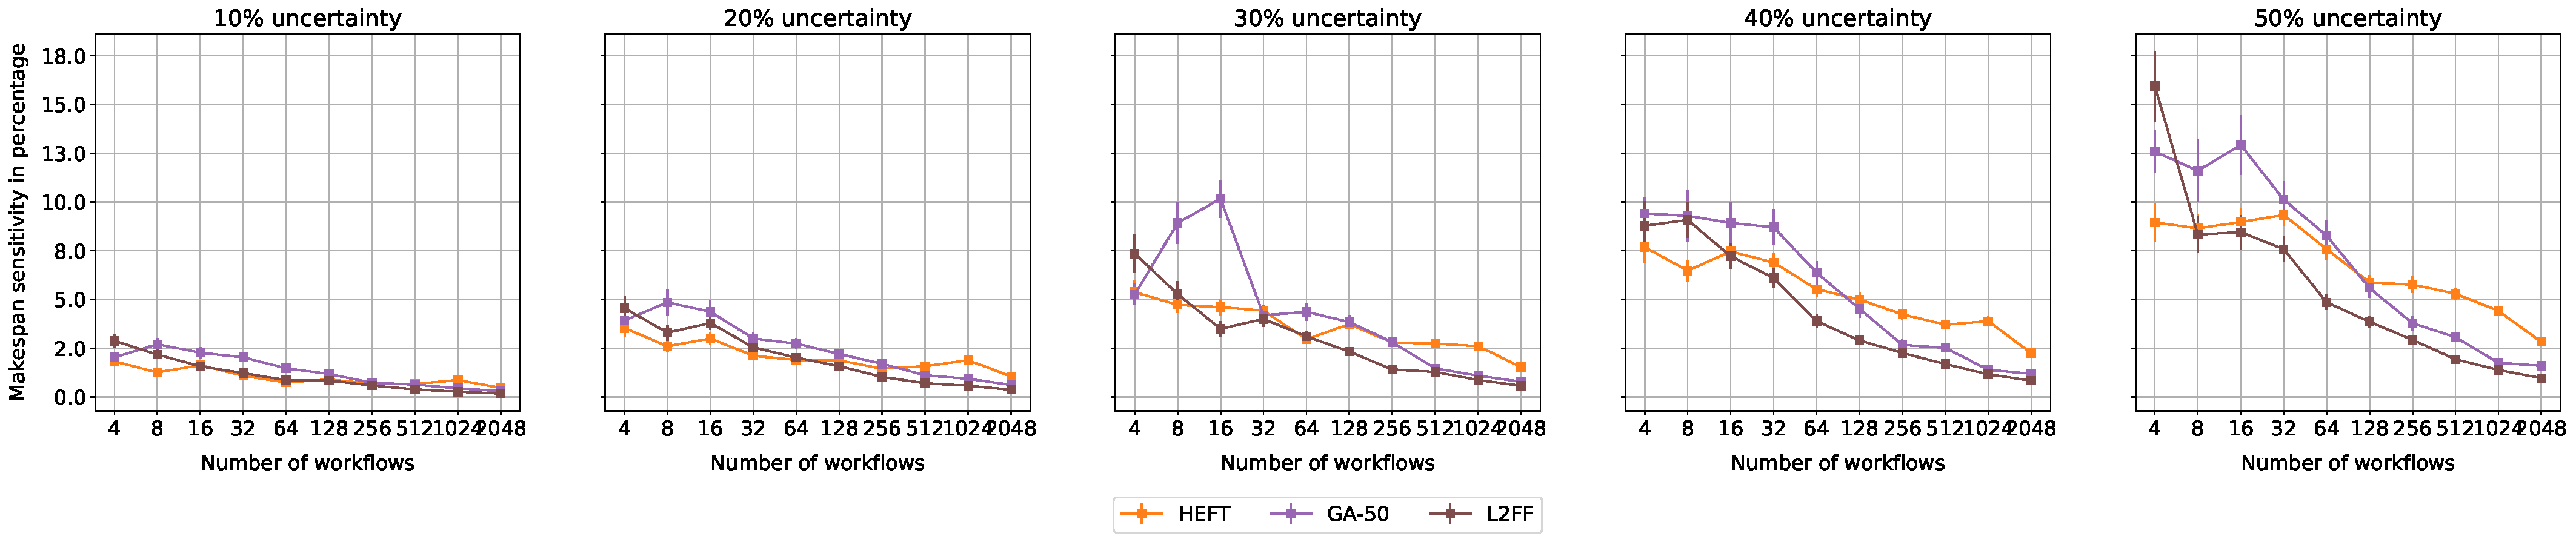
\includegraphics[width=.95\textwidth]{figures/campaign/InaccurStHeteroCampaigns_4StHeteroResourcesSens.pdf}
        \caption{}
        \label{fig:InaccurStHeteroCampaigns_4StHeteroResourcesSens}
    \end{subfigure}\\
    ~ 
    \begin{subfigure}[b]{0.85\textwidth}
        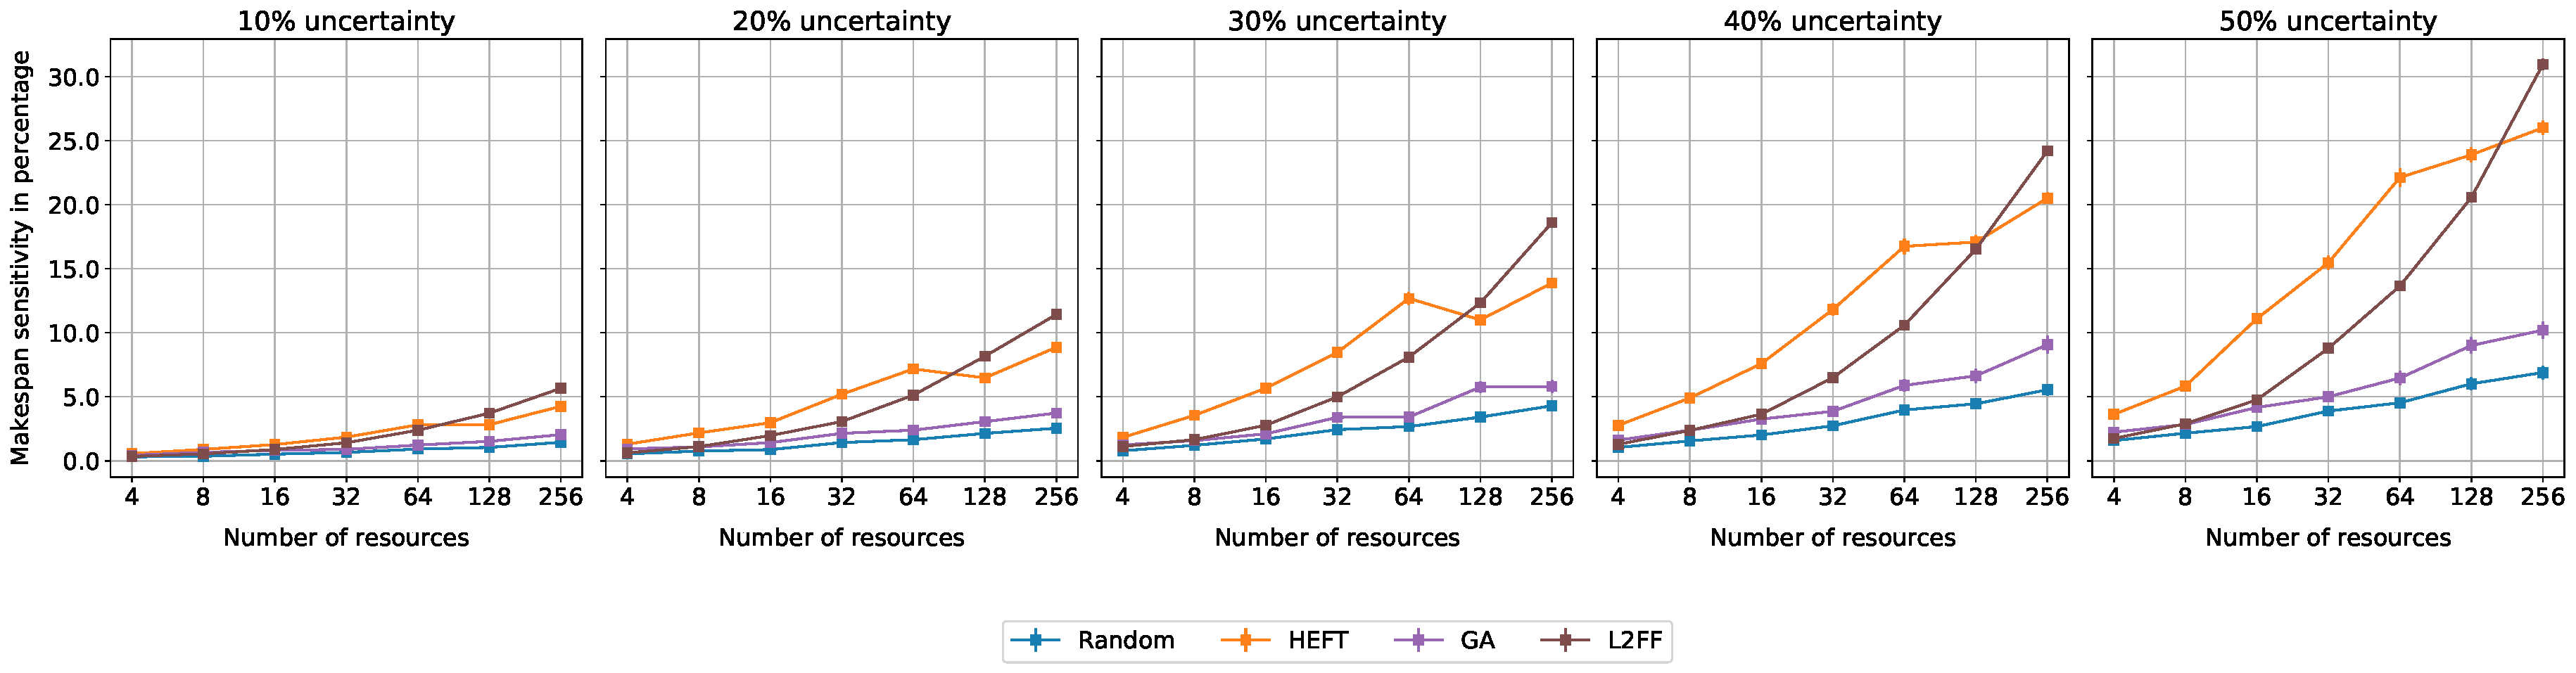
\includegraphics[width=0.95\textwidth]{figures/campaign/InaccurStHeteroResources_StHeteroCampaignsSens.pdf}
        \caption{}
        \label{fig:InaccurStHeteroResources_StHeteroCampaignsSens}
    \end{subfigure}
    \caption{~\ref{fig:InaccurStHeteroCampaigns_4StHeteroResourcesSens} Makespan sensitivity for different levels of uncertainty and different number of workflows on 4 heterogeneous resources;
    ~\ref{fig:InaccurStHeteroResources_StHeteroCampaignsSens} Makespan sensitivity for different levels of uncertainty and different number of resources for 1024 workflows static resources.}
    \label{fig:inaccur_st}
\end{figure}

As per our expectation, sensitivity to workflow uncertainty shows similar behavior to sensitivity to resource dynamism.
Sensitivity decreases when the number of workflows increase (Fig.~\ref{fig:InaccurStHeteroCampaigns_4StHeteroResourcesSens}) and increases as the number of resources increase (Fig.~\ref{fig:InaccurStHeteroResources_StHeteroCampaignsSens}).
This verifies our conclusion from experiment 2 that sensitivity is proportional to the number of resources and inverse proportional to the number of workflows.

Sensitivity to makespan runtime uncertainty shows a wide range of values for HEFT and L2FF, but significantly smaller range for GA-50 and random.
Specifically, the sensitivity of plans using HEFT is between almost 0~\% for 2048 workflows on 4 resource and 25~\% for 1024 workflows on 256 resources.
The sensitivity of plans using L2FF show similar range to HEFT with L2FF reaching 35~\% for 1024 workflows on 256 resources.
GA-50 plans show increased sensitivity for small number of workflows when the number of resources is constant, around 13~\%, and quickly drop close to 0~\%.

HEFT shows higher sensitivity than GA-50 and L2FF above 128 workflows/4 resources and when the number of resources change and the campaign size is 1024 workflows.
In addition, we see higher sensitivity for plans that use HEFT and L2FF than plans that use GA-50 when the number of resources increase.
Both HEFT and L2FF create priority lists for the workflows and GA-50 does not.
As a result, HEFT and L2FF place large workflows on less perfomant resources.
GA-50 does not prioritize workflows and places a subset of workflows to resources randomly.
As a consequence, the random order of the workflows with the random placement reduces the effect of the workflow runtime uncertainty.

This experiment studies how sensitive are plans using HEFT, GA and L2FF are when the workflow runtime estimation is uncertain.
Algorithms that prioritize workflows, HEFT and L2FF, tend to be more sensitive to workflow runtime estimation uncertainty than algorithms that do not create a priority list, GA and random.
HEFT and L2FF are more sensitive than GA-50 and random when the number of resources increase and show similar sensitivity to GA-50 and random when the number of workflows increase --- 25~\% and 35~\% compared to less than 10~\% for 1024 workflows and 256 resources.
In addition, sensitivity remains proportional to the number of resources and inverse proportional to the number of workflows.
This in conjunction with experiment 2 allows us to conclude that the sensitivity slope is independent from the type of uncertainty.


\section{Conclusions}
\label{sec:cf_algo_sel}
In this chapter, we discuss and compare planning algorithms to plan the execution of a computational campaign on HPC resources.
Specifically, we discuss three planning algorithms, HEFT, a genetic algorithm (GA) and L2FF, and their algorithmic characteristics.
Our experimental methodology allows us to compare plans in terms of makespan performance and their sensitivity to resource dynamism and workflow runtime uncertainty.

Based on our analysis, we conclude that there are three factors which affect the performance and sensitivity of planning algorithms.
The first factor is whether the algorithm uses an expectation of when a resource will be available.
HEFT and the genetic algorithm use an expectation of resource availability and show better performance on homogeneous and heterogeneous resources than L2FF and random.
The second factor is whether the algorithm uses a deterministic or randomized heuristic.
GA shows performance similar to random plans when all workflows were initially placed randomly to resources.
In addition, GA shows worse performance than L2Ff when 50~\% of the workflows were not placed randomly above 128 resources as it underutilized some of the resources.
The third factor is whether the algorithm creates a workflow priority list based on workflow runtime.
HEFT and L2FF sort workflows based on their runtime and they place first the larger workflows on their lists.
This priority list allows L2FF to place larger workflows to more performant resources and as a result L2Ff outperforms GA for large number of resources.

Our analysis on makespan sensitivity to resource dynamism also shows that deterministic algorithms are more sensitive to resource dynamism or workflow runtime uncertainty than non-deterministic algorithms.
HEFT and L2FF provide more sensitive plans than GA and random.
Further, sensitivity is proportional to the number of resources and inverse proportional to the number of workflows.
Sensitivity to resource dynamism or workflow runtime uncertainty decreases as the number of workflows increase when using constant number of resources and increases when number of resources increases and campaign size is constant.
When variation originates from workflow runtime uncertainty, both HEFT and L2FF were more sensitive than GA-50 since they prioritize workflows based on their runtime estimation.

When selecting a planning algorithm for a campaign, users should consider the following factors:
\begin{inparaenum}[1)]
    \item resource homogeneity/heterogeneity;
    \item resource dynamism; and
    \item workflow runtime estimation uncertainty.
\end{inparaenum}
When resources are homogeneous, a planner like L2FF provides a plan with good makespan, is very simple to engineer and is not significantly more sensitive from algorithms like HEFT or GA.
When resources are heterogeneous and the computational objective is to produce the best possible makespan, an algorithm which is deterministic, produces information about resource availability and creates a priority list, such as HEFT is a good candidate.
If the computational objective of a campaign is to use a plan that is not very sensitive to resource dynamism or workflow runtime uncertainty, a non-deterministic algorithm, like a genetic algorithm, is a good candidate.
Although a genetic algorithm may not provide worse makespan than an algorithm like HEFT, its plans are less sensitive to variations.


%% --------------------------------- OLD TEXT ----------------------------------

%% ---------------------------- HEFT EXTENSION ---------------------------------
%HPC resources may become unavailable for multiple reasons, including but not limited to maintenance, a random failure, executing a workflows over the expected time., etc.
%In order to be able to utilize HEFT for dynamic resources, we had to extend Algorithm~\ref{alg:heft} to take as input the time that a resource is initially available.
%This input can be represented as a dictionary where the keys are the available resources and the values are the time a resource becomes available.
%The extended algorithm is shown in Algorithm~\ref{alg:ext_heft}.
%Although the extension may be small, it is crucial to allow to reuse HEFT based on the state of the execution at a given point in time.
%
%\begin{algorithm}[ht]
%    \caption{Extended Heterogeneous Earliest Finish Time (EHEFT) algorithm}
%    \label{alg:ext_heft}
%    \begin{algorithmic}[1]
%        \Procedure{EHEFT}{$W$, $R$, $T$}\Comment{$W$ and $R$ are a set of workflow and resources respectively. $T$ is a dictionary of when a resource becomes available.}
%        \State \texttt{Calculate the computation cost $w_{tx}^{ij}$ of each workflow for all resources}
%        \State \texttt{Assign $rank_i = \overline{w_{i}} = \nicefrac{\sum_{j=1}^{|R|}w_{tx}^{ij}}{|R|}$}
%        \State \texttt{Sort workflows by non-increasing order of $rank_i$}
%        \While{unscheduled workflows}
%        \State \texttt{Select the first workflow $\tilde{w}$ from the sorted list}
%        \For{$\forall r_{j}$ in $R$}
%        \State\texttt{Compute earliest finish time for $\tilde{w}$ on $r_{j}$ based on $T(r_j)$, $eft_{\tilde{w},r_j}$ }
%        \EndFor
%        \State \texttt{Assign  $\tilde{w}$ on $r_k$ with $\min{(eft_{\tilde{w},r_j})}$}
%        \EndWhile
%        \EndProcedure
%    \end{algorithmic}
%\end{algorithm}
%

%% -------------------- GA EXTENSION -------------------------------------------
%We extend this algorithm in the population initialization to support replanning..
%The initialization method takes into account the times resources will be available during for the EFT heuristic.
%Another point of extension would be the fitness function.
%However, the fitness function of the selected algorithm~\cite{page2005algorithm} already takes into account the previous load of a resource, which is the time a resource is available.

%% -----------------------------------------------------------------------------
%In figure~\ref{fig:dyn_hetero_homog_sens_analysis} we introduce workflow heterogeneity.
%The algorithms makespan performance behavior is similar to the one shown in Fig.~\ref{fig:het_het_analysis}.
%Despite the fact, HEFT show the largest sensitivity when varying the number of workflows and when varying the number of resources.
%The genetic algorithm shows similar sensitivity with HEFT when the number of workflows but tends to be less sensitive when the number of resources increase.
%The genetic algorithm assigns a percentage of workflows to resources randomly which in turn makes it less sensitive to resource dynamicity, especially when the number of resources is large.

%L2FF shows a similar behavior with HEFT, especially when the number of resources changes, despite being less sensitive.
%In addition, the genetic algorithm sensitivity gets closer to that of random when the number of resources increases.
%Both L2FF and HEFT are deterministic and they produce always the same plan for a given campaign and set of resources.
%This in turn results to an increasing sensitivity as the ratio of number of campaign size to number of resources is small.
%In contrast, the random initial placement of GA allows it to create a plan that is less sensitive to dynamicity with the cost of slightly makespan, 725K seconds versus 643K and 649K seconds from HEFT and L2FF respectively.

%% -----------------------------------------------------------------------------
% Experiment 3 dynamic resources
%
%The ratio of number of workflows over the number of resources remains inverse proportional to the sensitivity.
%In addition, specifically for HEFT the impact of uncertainty increases significantly as the number of resources increase, reaching 55~\%.
%Since HEFT places one or two workflows on these resources, any change affects significantly its expected makespan.
%This verifies our conclusion from experiment 2, that algorithms with strong assumptions about workflow runtime and resource availability are very sensitive to changes.
%
%Introducing resource dynamism increased further the sensitivity of the algorithms, as seen in figure~\ref{fig:inaccur_dyn}.
%The observed increase was no more than the level shown in experiment 2.
%This shows us that the overall sensitivity is the summation of independently measured sensitivity from different sources.
%
%The results of our experiments show that algorithms which make significant assumptions about the workflow length and resource performance produce better makespan.
%That is apparent from the fact that HEFT consistently produces the smaller makespan.
%This is true also when resources are dynamic and the workflows runtime is uncertain even at 90~\%.
%HEFT had a sensitivity of around 60~\% maximum which is not enough to affect the plan in such a way that another algorithm would be preferable.
%Furthermore, knowledge of resource heterogeneity and availability is an important factor in differentiating the performance of the algorithms, as seen by the performance difference of L2FF compared to HEFT and GA.
%Lastly, the ratio of the number of workflows over the number of resources affects the level of sensitivity of the algorithms.
%The less number of workflows placed on resources higher the significance of a change either in the performance of the resources or the workflow runtime.
%

%% -----------------------------------------------------------------------------
%
%\subsection{Experiment 4: Performance Gain using Plan Adaptation}
%
%An adaptive plan is a new plan derived from the previous one on the base of information acquired at runtime.
%Plan adaptation can happen either via running the planning algorithm again with the new information or via submitting a workflow to the selected resource when it becomes available.
%In this experiment, we focus on the second type of adaptation since L2FF does not know when exactly a resource becomes available.
%Specifically, when a resource becomes available earlier than expected, the bookkeeping component pushes the next workflow to the selected resource, otherwise the workflow is queued and executes as soon the resource becomes available.
%
%We measure the performance gain of adaptive plans for executing a campaign with heterogeneous workflows and different level of uncertainty on heterogeneous dynamic resources.
%Figure~\ref{fig:gain_dyn} shows the normalized performance gain as a function of the workflow runtime uncertainty and either the number of workflows, fig.~\ref{fig:InaccurStHeteroCampaigns_4DynHeteroResourcesGain}, or the number of resources, fig.~\ref{fig:InaccurDynHeteroResources_StHeteroCampaignsGain}.
%As we can see the performance gain is not significant.
%L2FF adaptive plan shows a maximum of 16~\% for 4 workflows and 4 resources, GA and HEFT around 12~\%, while when the number of resources vary none of the plans exceeds 6~\%.
%
%
%\begin{figure}[ht!]
%    \centering
%    \begin{subfigure}[b]{0.95\textwidth}
%        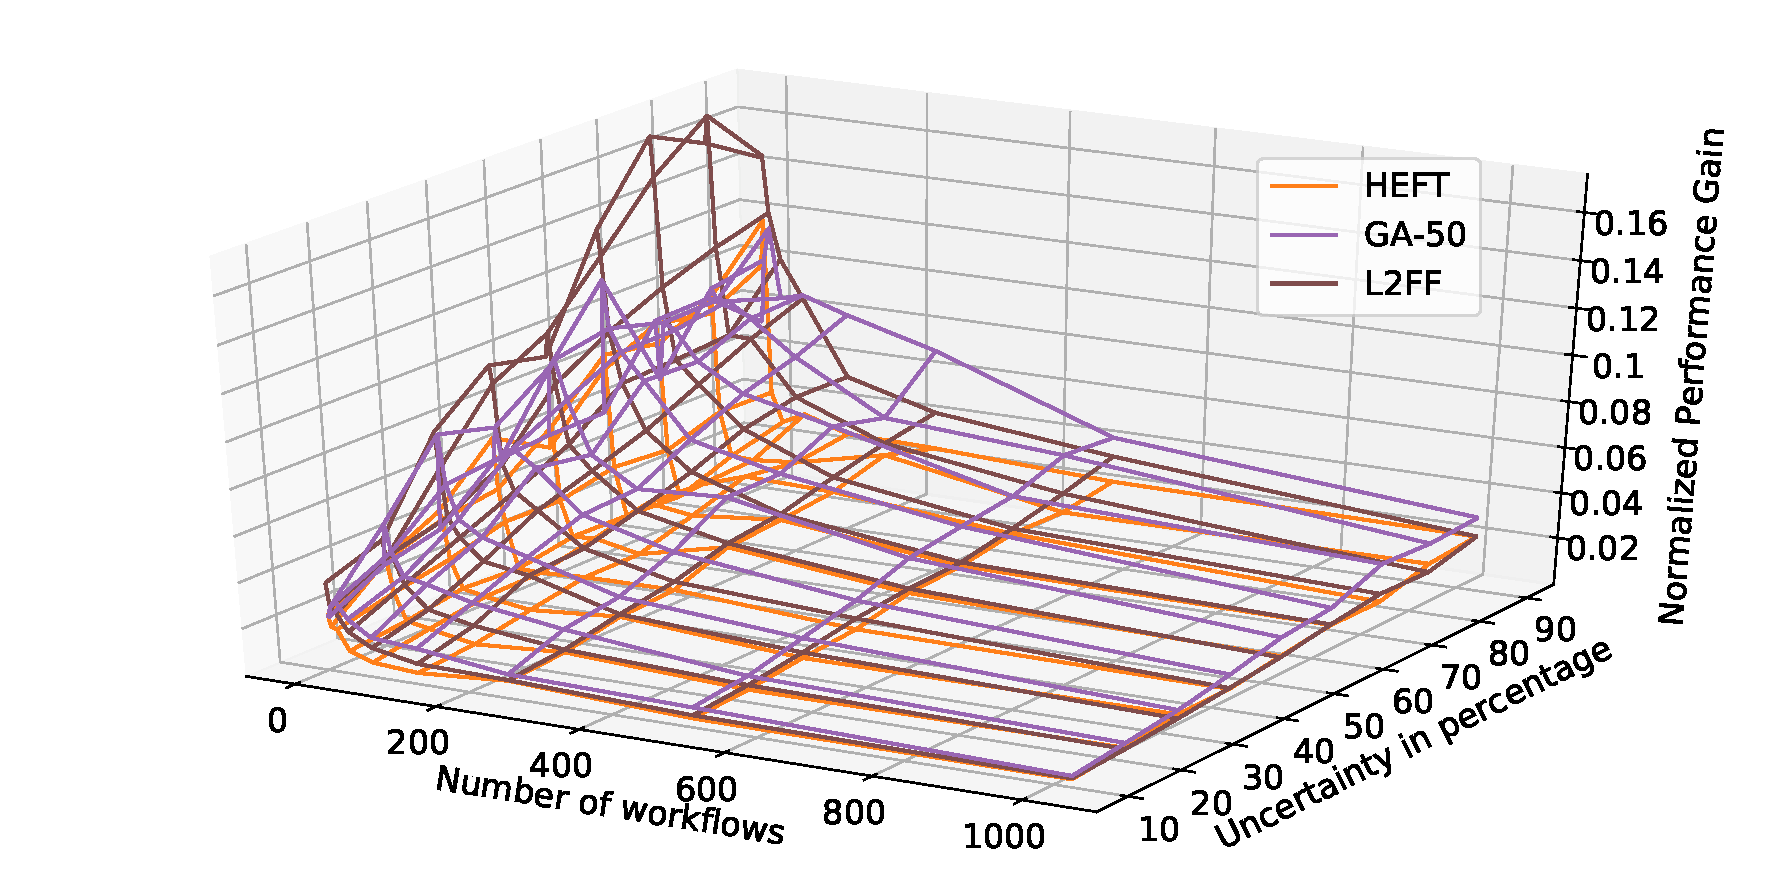
\includegraphics[width=.95\textwidth]{figures/campaign/InaccurStHeteroCampaigns_4DynHeteroResourcesGain.pdf}
%        \caption{}
%        \label{fig:InaccurStHeteroCampaigns_4DynHeteroResourcesGain}
%    \end{subfigure}\\
%    ~ 
%    \begin{subfigure}[b]{0.95\textwidth}
%        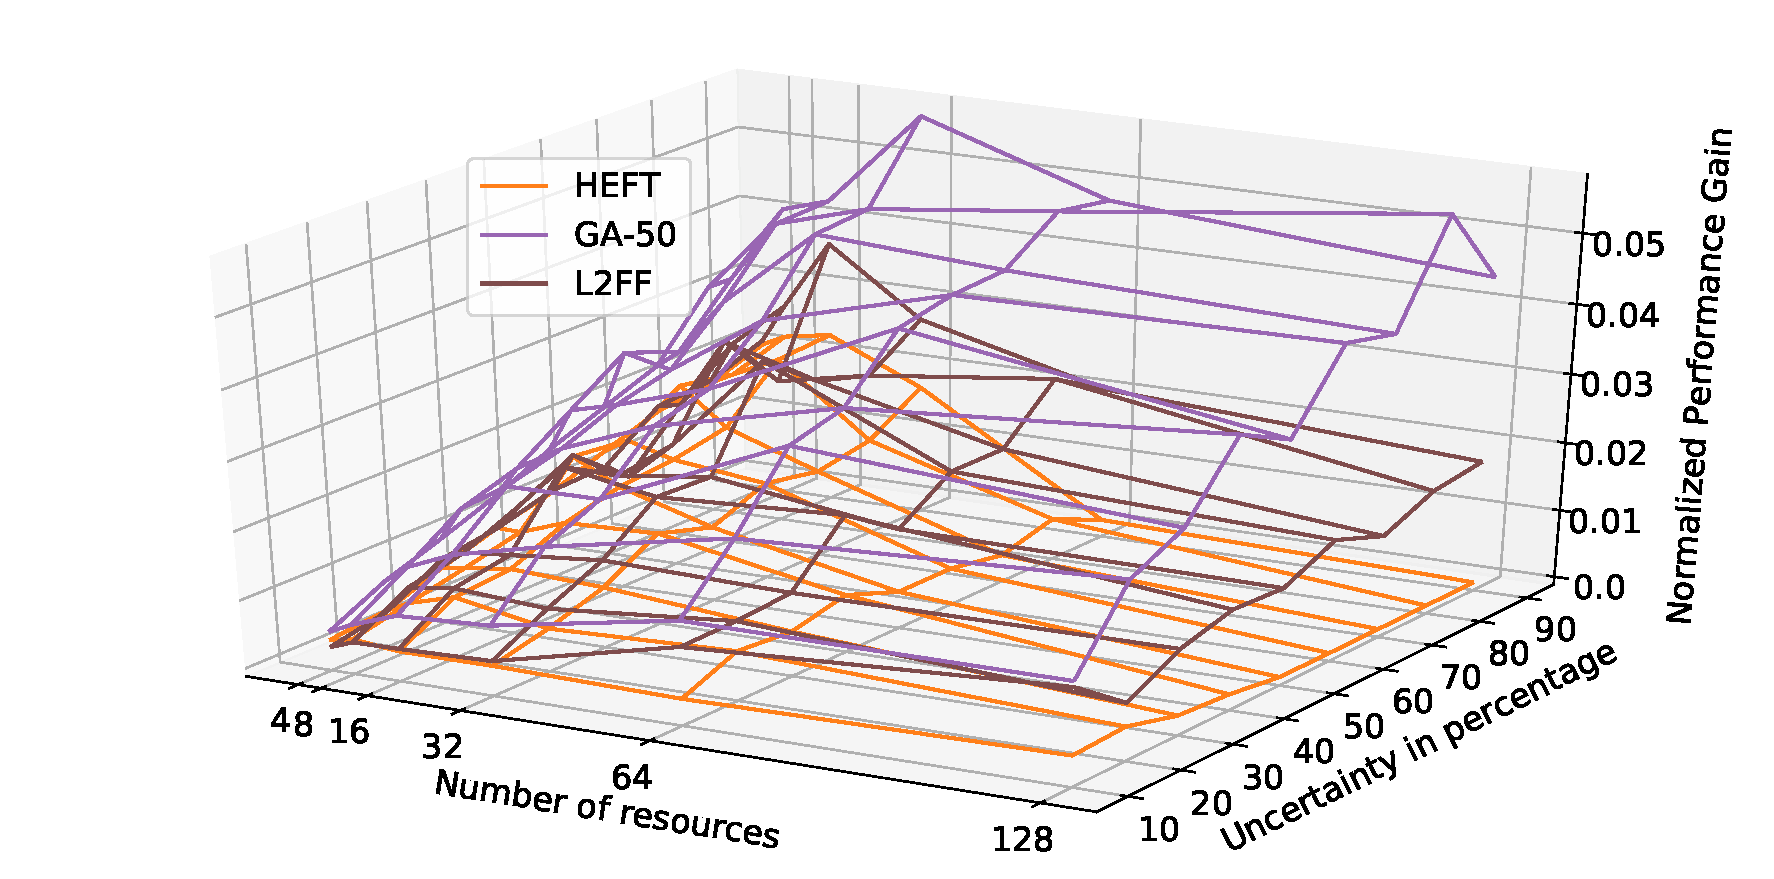
\includegraphics[width=0.95\textwidth]{figures/campaign/InaccurDynHeteroResources_StHeteroCampaignsGain.pdf}
%        \caption{}
%        \label{fig:InaccurDynHeteroResources_StHeteroCampaignsGain}
%    \end{subfigure}
%    \caption{~\ref{fig:InaccurStHeteroCampaigns_4DynHeteroResourcesGain} Normalized performance gain for different levels of uncertainty and different number of workflows on static resources;
%        ~\ref{fig:InaccurDynHeteroResources_StHeteroCampaignsGain} Normalized performance gain for different levels of uncertainty and different number of resources on static resources.}
%    \label{fig:gain_dyn}
%\end{figure}
%
%Since adaptive plans try to mitigate the effects of resource dynamism and workflow runtime uncertainty, we expect that the performance gain would be proportional to the ratio of number of workflows over the number of resources.
%Although this is generally true for L2FF and GA, it is not for HEFT.
%This is due to the fact that HEFT is placing a small number, 1 or 2, of workflows on slow resources.
%As a result, adaptive plans have no or very little effect.
%Contrary, L2FF and GA place more workflows on the slow resources allowing the adaptation to provide some gains.


%% --------------------------- Last Experiment ---------------------------------

%\begin{figure}[ht!]
%    \centering
%    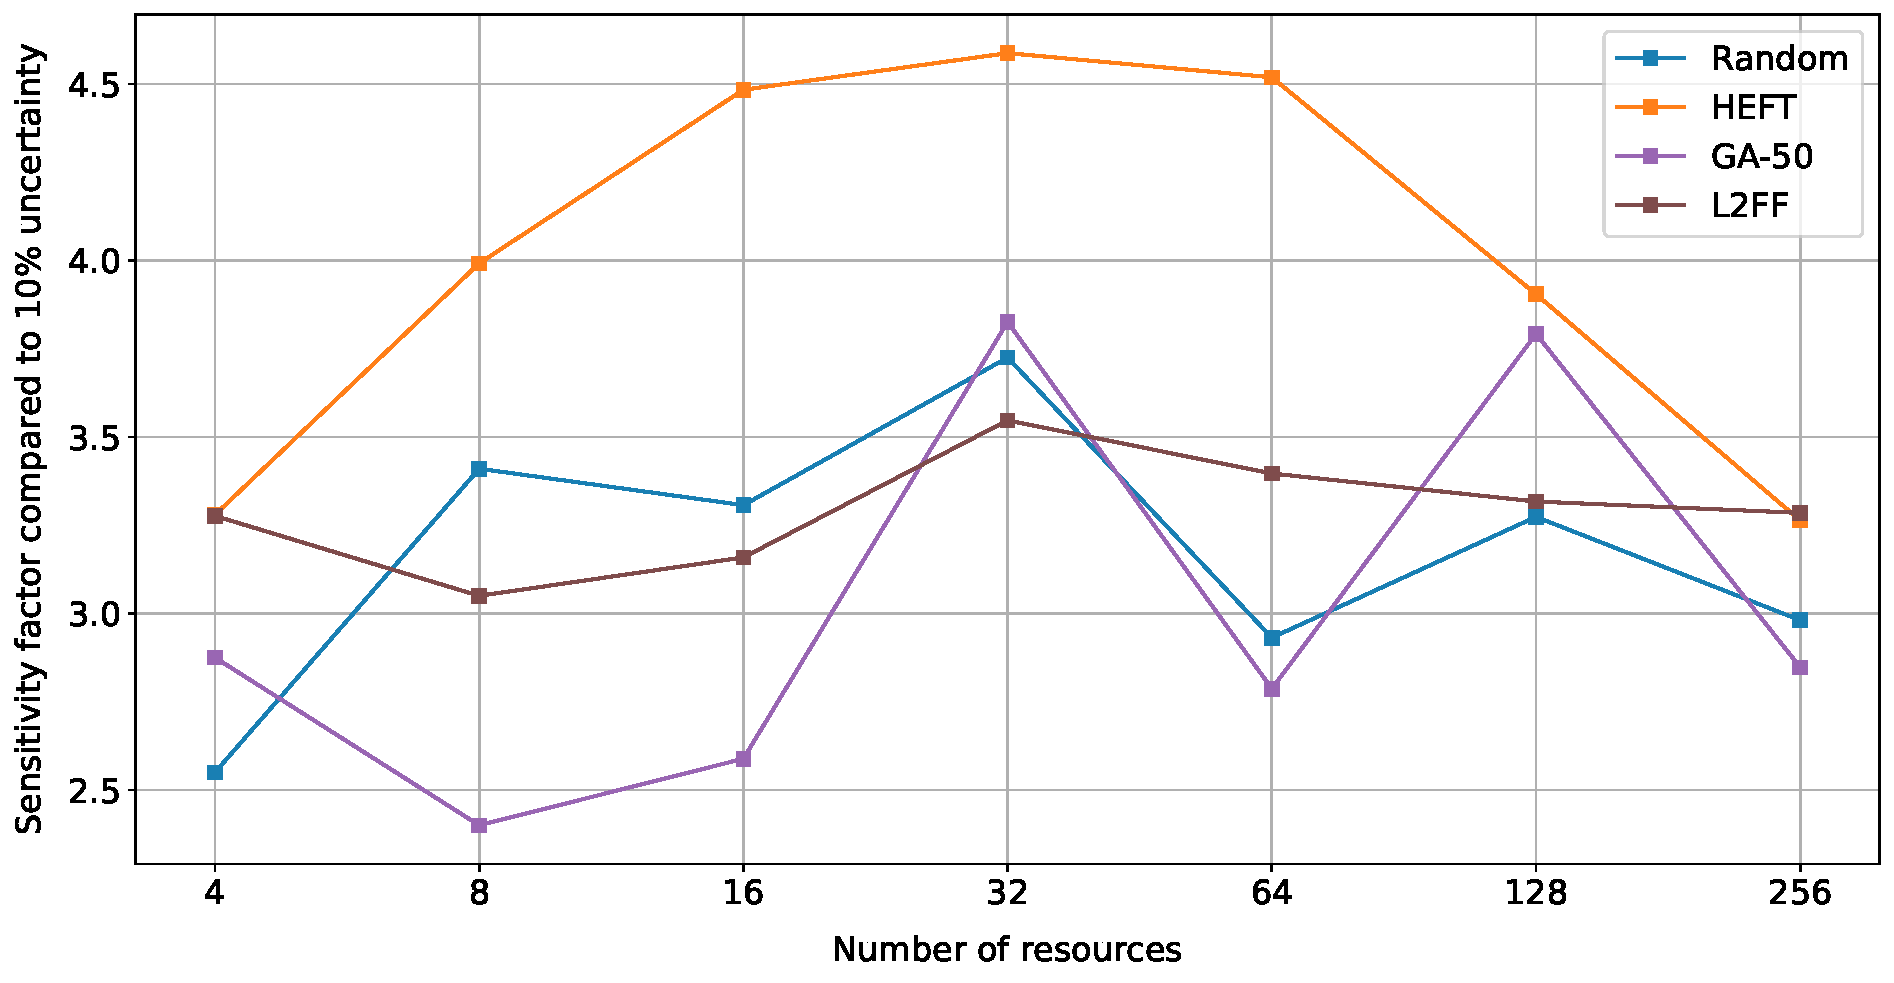
\includegraphics[width=.95\textwidth]{figures/campaign/InaccurStHeteroResources_StHeteroCampaignsSensFactor.pdf}
%    \caption{Sensitivity factor for 30~\% uncertainty compared to 10~\% uncertainty for different number of resources and 1024 workflows.}
%    \label{fig:InaccurStHeteroResources_StHeteroCampaignsSensFactor}
%\end{figure}

%As the level of uncertainty increases the sensitivity increases proportionally for L2FF and GA-50 and not for HEFT regardless of whether the number of workflows or the number of resources changes.
%HEFT shows an increase larger than the expected multiplicative factor when the number of workflows over the number of resources is between 8 and 128.
%As an example, figure~\ref{fig:InaccurStHeteroResources_StHeteroCampaignsSensFactor} shows the increase factor of 30~\% uncertainty compared to 10~\% for different number of resources and 1024 workflows.
%L2FF, GA-50 and random increase is relatively close to 3 compared to the increase observed for HEFT which reaches more than 4 times.
%We believe that this unexpected behavior from HEFT is a consequence of prioritizing workflows and placing a workflow on the resource that will finish it earlier.